\documentclass[journal]{IEEEtranTIE}
\usepackage{graphics} % for pdf, bitmapped graphics files
\usepackage{epsfig} % for postscript graphics files
\usepackage{subcaption}
\usepackage[noadjust]{cite}
\usepackage{algorithm,algpseudocode}
\usepackage{gensymb} % enable the use of degree symbol
\usepackage{amsmath,amssymb,amsfonts,amsthm} % assumes amsmath package installed

% format for theorems etc.
\newtheorem{thm}{\bfseries Theorem}
\newtheorem{lem}{\bfseries Lemma}
\newtheorem{cor}{\bfseries Corollary}
\newtheorem{prop}{\bfseries Proposition}
\theoremstyle{remark}
\newtheorem{rem}{\bfseries Remark}
%\newtheorem*{proof*}{\bfseries Proof}

% format for argmin, argmax
\newcommand{\argmax}{\operatornamewithlimits{argmax}}

% format for cross-reference
\usepackage[capitalize]{cleveref}
\crefname{equation}{eq.}{eq.}
\Crefname{equation}{Eq.}{Eq.}
\crefname{thm}{theorem}{theorems}
\Crefname{thm}{Theorem}{Theorems}
\crefname{lem}{lemma}{lemmas}
\Crefname{lem}{Lemma}{Lemmas}
\crefname{cor}{corollary}{corollaries}
\Crefname{cor}{Corollary}{Corollaries}
\crefname{prop}{proposition}{propositions}
\Crefname{prop}{Proposition}{Propositions}
\crefname{rem}{remark}{remarks}
\Crefname{rem}{Remark}{Remarks}

%=====todonotes===== %
\usepackage{todonotes}
\usepackage{soul}
\definecolor{smoothgreen}{rgb}{0.7,1,0.7}
\sethlcolor{smoothgreen}

\newcommand{\todopara}[1]{\vspace{0px} %
	\todo[inline, color=black!10]{\textbf{[Paragraph:]} {#1}} %
}
\newcommand{\todonote}[1]{\vspace{0px} %
	\todo[inline, color=green!30]{\textbf{[Note:]} {#1}} %
}
\newcommand{\todoQ}[1]{\vspace{0px} %
	\todo[inline, color=orange!50]{\textbf{[Note:]} {#1}} %
}
\newcommand{\todohere}[1]{\hl{(\textbf{TODO:} #1)}}

\newcommand{\hidetodos}{
	\renewcommand{\todopara}[1]{}
	\renewcommand{\todonote}[1]{}
	\renewcommand{\todoQ}[1]{}
	\renewcommand{\todohere}[1]{}
}


%---------- Macros for this paper
% random variables
\newcommand{\X}{X}
\newcommand{\Z}{Z}
\newcommand{\xg}{x^g}

\title{\LARGE \bf
	Measurement Dissemination-based Distributed Bayesian Filter using the Latest-In-and-Full-Out Exchange Protocol for Networked Unmanned Vehicles}

\author{Chang Liu, Shengbo Eben Li and J. Karl Hedrick% <-this % stops a space
	\thanks{*The first two authors, C. Liu and S. Li, have equally contributed to this research. All correspondence should be addressed to S. Li. The work is supported by the ONR MURI project and the NSF China with grant 51575293 and 51622504.}
%	}% <-this % stops a space
%	\thanks{$^{1}$C. Liu and J. Hedrick are with the Department of Mechanical Engineering, University of California, Berkeley, Berkeley, CA 94709, USA. Email: {\tt\small changliu@berkeley.edu, khedrick@me.berkeley.edu}}%
%	\thanks{$^{2}$S. Li is now with the Department of Automotive Engineering, Tsinghua University, Beijing, 100084, China. He has worked at the Department of Mechanical Engineering, University of California, Berkeley. Email: {\tt\small lisb04@gmail.com}}
}

\begin{document}
	
	%\hidetodos % hide all todos 
	
	\maketitle
	\thispagestyle{empty}
	\pagestyle{empty}
	
	%\setlength{\belowcaptionskip}{-10pt} % set the spacing between figure and text
	
	%%%%%%%%%%%%%%%%%%%%%%%%%%%%%%%%%%%%%%%%%%%%%%%%%%%%%%%%%%%%%%%%%%%%%%%%%%%%%%%%
	\begin{abstract}
		This paper presents a measurement dissemination-based distributed Bayesian filter (DBF) for a network of unmanned ground vehicles (UGVs).
		The DBF utilizes the Latest-In-and-Full-Out (LIFO) exchange protocol to disseminate the sensor measurements within local neighbors.
		Different from existing statistics dissemination strategies that transmit posterior distributions or likelihood functions, each UGV under LIFO only exchanges
		latest available measurements,
		which significantly reduces the transmission burden between each pair of UGVs to scale linearly with the network size.
		Under the condition of fixed and undirected topology, LIFO can guarantee non-intermittent dissemination of all measurements over the network within a finite time.
		Two types of LIFO-based DBF algorithms are then derived to estimate individual probability density function (PDF) of the static target and moving target, respectively. 
		For the former, each UGV locally fuses the newly received measurements, while for the latter, a set of measurement history is stored and sequentially fused. 
		The consistency of LIFO-based DBF is proved that the estimated target position converges in probability to the true target position.
		The effectiveness of this method is experimentally demonstrated by the target localization via multiple mobile robots with sonar sensors in an indoor environment.
	\end{abstract}
	
	\begin{IEEEkeywords}
		Bayesian filter, Distributed estimation, Networked vehicles, Nonlinear filter, Unmanned vehicles.
	\end{IEEEkeywords}
	%%%%%%%%%%%%%%%%%%%%%%%%%%%%%%%%%%%%%%%%%%%%%%%%%%%%%%%%%%%%%%%%%%%%%%%%%%%%%%%%
	\section{INTRODUCTION}
	Distributed filtering that focuses on using a group of networked UGVs to collectively infer environment status has been used for various applications, such as intruder detection \cite{chamberland2007wireless}, moving target tracking \cite{wang2012cooperative} and object localization \cite{song2012mobile}. 
	Several techniques have been developed for distributed filtering.
	For example, Olfati-Saber (2005) proposed a distributed Kalman filter (DKF) for estimating states of linear systems with Gaussian process and measurement noise \cite{2005distributed}.
	Each DKF used low-pass and band-pass consensus filters to compute the average of weighted measurements and inverse-covariance matrices.
	Madhavan et al. (2004) presented a distributed extended Kalman filter for nonlinear systems \cite{madhavan2004distributed}.
	This filter was used to generate local terrain maps by using pose estimates to combine elevation gradient and vision-based depth with environmental features.
	Gu (2007) proposed a distributed particle filter for Markovian target tracking over an undirected sensor network \cite{gu2007distributed}. 
	Gaussian mixture models (GMM) were adopted to approximate the posterior distribution from weighted particles, and the parameters of GMM were exchanged via average consensus filter.
	As a generic filtering scheme for general system dynamics and arbitrary noise distributions, distributed Bayesian filters (DBF) have received increasing interest during past years \cite{bandyopadhyay2014distributed,julian2012distributed}, which are also the focus of this study.
	It is worth noting that Bayesian filters can be reduced to Kalman filters and particle filters under appropriate conditions \cite{chen2003bayesian}.
	
	The design of distributed filtering algorithms depends on the communication topology of a multi-UGV network, which can be classified into two types: fusion center (FC)-based and neighborhood (NB)-based.
	In the FC-based approaches, each UGV uses a filter to estimate local statistics of environment status based on its own measurement.
	The local statistics are transmitted (possibly via multi-hopping) to a single FC, where a global posterior distribution (or statistical moments in DKF \cite{olfati2007consensus}) is calculated at each filtering cycle after receiving all local information \cite{zuo2006bandwidth,he2014networked}.
	In the NB-based approaches, a set of UGVs executes distributed filters to estimate individual posterior distribution. 
	The consensus of individual estimates is achieved by solely communicating statistics and/or measurements within local neighbors.
	The NB-based methods have become popular in recent years, since such approaches do not require complex routing protocols and global network knowledge and are therefore rather robust to topological changes and link failures.
	
	So far, most studies on NB-based distributed filtering have focused on the so-called \textit{statistics dissemination} strategy.
	This strategy directly exchanges environment statistics, including posterior distributions and likelihood functions, within neighboring UGVs \cite{hlinka2013distributed}.
	It can be further categorized into two types: leader-based and consensus-based. 
	In the former, statistics are sequentially passed and updated along a path formed by active UGVs, called leaders.
	Only the leaders can perform filtering based on its own and the received measurements from local neighbors.
	For example, Sheng et al. (2005) proposed a multiple leader-based distributed particle filter with Gaussian Mixer for target tracking \cite{sheng2005distributed}. 
	Sensors are grouped into multiple uncorrelated cliques, in each of which a leader is assigned to perform particle filtering and exchanges particle information with other leaders.
	In the consensus-based distributed filters, every UGV diffuses environment statistics among neighbors, via which the global agreement of the statistics is achieved by using multi-agent consensus laws \cite{olfati2007consensus,ren2005consensus,jadbabaie2003coordination}.
	For example, Hlinka et al. (2012) proposed a distributed method for computing an approximation of the joint (all-sensors) likelihood function by means of weighted-linear-average consensus algorithm when local likelihood functions belong to the exponential family of distributions \cite{hlinka2012likelihood}.
	Saptarshi et al. (2014) presented a Bayesian consensus filter that uses a logarithmic opinion pool for fusing posterior distributions of the tracked target \cite{bandyopadhyay2014distributed}.
	Other examples can be found in \cite{julian2012distributed} and \cite{beaudeau2012target}.
	
	Despite the popularity of environment statistics dissemination strategies, exchanging statistics can consume excessive communication resources.
	One promising remedy is to disseminate sensor measurement instead of environment statistics among neighbors.
	One early work was done by Coates et al. (2004), which used adaptive encoding of sensor measurements to minimize communication overhead \cite{coates2004distributed}.
	A recent study was conducted by Djuric et al. (2011), which proposed to broadcast raw measurements to other agents, and therefore each UGV had a complete set of measurements of other UGVs for executing particle filtering \cite{djuric2011non}.
	A shortcoming of aforementioned works is that their communication topologies are assumed to be a complete graph: 
	a UGV can directly exchange information with any other UGV via a single hopping even they are far from each other. This is a strong assumption on the communication network and is not always feasible in reality \cite{jadbabaie2003coordination,bandyopadhyay2014distributed}.
	For incomplete graphs, Leung et al. (2010) explored a decentralized filter for dynamic robot networks \cite{leung2010decentralized}.
	The algorithm was shown to achieve centralized-equivalent filtering performance in simulations. 
	However, it required the communication of both measurements and statistics, which incurred large communication overhead.
	
	\textcolor{black}{In this work, we propose a novel measurement dissemination-based distributed Bayesian filtering approach for target localization using networked UGVs.
		The main contributions of this paper include:
		(a) Different from existing works that assume full connectivity of the communication topology, each UGV only needs to broadcast the sensor measurements to its neighbors via single hopping and then implements individual Bayesian filter locally using its own measurements and the ones transmitted from neighbors.
		(b) We introduce the Latest-In-and-Full-Out (LIFO) protocol to reduce the communication burden,
		with the transmission data scaling linearly with the UGV number.
		(c) The proposed LIFO-based DBF has the following properties: For a fixed and undirected network, LIFO guarantees the global dissemination of measurements over the network in a non-intermittent manner.
		The corresponding DBF ensures the consistency of estimated target position, i.e., the estimate converges in probability to the true value when the number of measurements tends to infinity.}
	
	The rest of this paper is organized as follows: 
	The problem of distributed Bayesian filtering is formulated in \cref{sec:prob_form}.
	The LIFO-based DBF algorithm is described in \cref{sec:LIFO-dbf}, followed by the proof of consistency in \cref{sec:consist_proof}.
	Simulation and experiment results are presented in \cref{sec:sim} and \cref{sec:exp}, respectively.
	The \cref{sec:conclu} concludes the paper.
	
	\section{PROBLEM FORMULATION}\label{sec:prob_form}
	Consider a network of $N$ UGVs to localize a target in a bounded two-dimensional space $S\in\mathbb{R}^{2}$. 
	Each UGV is equipped with a sensor for environment perception. 
	Due to the limit of communication range, each UGV can only share information 
	with its local neighbors.
	The Bayesian filter is run on each UGV based on its own measurements and the measurements of other UGVs to estimate the target position.
	
	\subsection{Target and Sensor Model}
	The target motion takes a deterministic discrete-time model: 
	
	\begin{equation}
		\small
		\label{eqn:tar_motion_model}
		\xg_{k+1}=f(\xg_k)
	\end{equation}\normalsize
	where the superscript $g$ represents the target; $\xg_k\in S$ is the target position at time $k$. % and $u^g_k$ is the target control input.
	
	The sensor measurement is described by a stochastic model:
	\begin{equation}\label{eqn:meas_model}
		z^i_k = h_i(\xg_k,x^i_k)+w^i_k,
	\end{equation}
	where the superscript $i\in\left\lbrace 1,\dots,N\right\rbrace$ represents the index of each UGV; $x^i_k\in S$ is the sensor position and $w^i_k$ is the white measurement noise.
	The measurement function $h_i$ depends on the type of the sensor.
	
	The information of the conditional probability of a certain measurement $z^i_k$ is critical to designing the updating procedure of a Bayesian filter \cite{thrun2005probabilistic}. 
	The conditional probability of $z^i_k$ given the sensor state $x^i_k$ and target state $\xg_k$ is denoted as $P(z^i_k|x^g_k;x^i_k)$, which depends on the distribution of the measurement noise.
	For example, if $w^i_k$ is a zero-mean Gaussian white noise with covariance $\Gamma_k^i$, then, according to \Cref{eqn:meas_model}, $P(z^i_k|x^g_k;x^i_k)$ can be described as
	\small\begin{equation*}
		P(z^i_k|x^g_k;x^i_k)=\mathcal{N}(h_i(\xg_k,x^i_k),\Gamma_k^i)\footnote{For the purpose of simplicity, we will not explicitly write the parameter $x^{i}_k$ in $P(z^i_k|x^g_k;x^i_k)$ for the rest of the paper.}.
	\end{equation*}\normalsize
	For non-Gaussian noise distributions, such as the Poisson noise or Cauchy noise \cite{kitagawa1996monte}, $P(z^i_k|x^g_k)$ can also be defined.
	It should be noted that, the approaches presented in this work do not rely on specific distributions of noise.
	
	\textcolor{black}{The $h_i$ of several typical sensors are defined as follows \cite{bishop2010optimality}:}
	
	\textcolor{black}{\textbf{Range-only sensors:} $h_i(\xg_k,x^i_k)=\|\xg_k-x^i_k\|_2$, where $\|\cdot\|_2$ is the Euclidean distance in $S$.}
	
	\textcolor{black}{\textbf{Bearing-only sensors:}
		$h_i(\xg_k,x^i_k)=\measuredangle (\xg_k-x^i_k)$,
		where $\measuredangle$ denotes the angle from the sensor to the target.}
	
	\textcolor{black}{\textbf{Range-bearing sensors:} $h_i(x^g_k,x^i_k)=x^g_k-x^i_k$.}
	
	\begin{rem}
		Given the knowledge of current target and UGV positions, current measurement by each UGV can be considered conditionally independent from its own past measurements and those by other UGVs \cite{bourgault2003optimal}.
	\end{rem}
	
	\subsection{Graphical Model of Communication Topology}
	The UGV network is assumed to be connected, i.e., there exists a path, either direct or indirect, between every pair of UGVs.
	Under this assumption, consider an undirected and fixed graph $G=(V,E)$, where $V=\left\lbrace 1,\dots,N\right\rbrace $ represents the index set of UGVs and $E=V\times V$ denotes the edge set. 
	The adjacency matrix $A=\left[ A_{(ij)}\right] $ describes the communication topology of $G$:
	\small\begin{equation*}
		A_{(ij)}=\begin{cases}
			1& \text{if}\;\left(i,j\right)\in E\\
			0& \text{if}\;\left(i,j\right)\notin E
		\end{cases},
	\end{equation*} \normalsize
	where $A_{(ij)}$ denotes the entity of the adjacency matrix. 
	The notation $A_{(ij)}=1$ indicates that a communication link exists between $i^\text{th}$ and $j^\text{th}$ UGV and $A_{(ij)}=0$ indicates no direct communication between them.
	
	The \textit{direct neighborhood} of $i^\text{th}$ UGV is defined as $\mathcal{N}_i=\left\lbrace j|A_{(ij)}=1,\forall j\in\left\lbrace1,\dots,N \right\rbrace \setminus \left\lbrace i \right\rbrace\right\rbrace $. 
	All the UGVs in $\mathcal{N}_i$ can directly exchange information with $i^\text{th}$ UGV via single hopping.  
	We also define another set $\mathcal{Q}_i$, called \textit{available neighborhood}, that contains indices of UGVs whose measurements can be received by the $i^\text{th}$ UGV via single or multiple hoppings.
	Therefore $\mathcal{N}_i\subseteq\mathcal{Q}_i$.
	\cref{fig:com_topo} illustrates three types of typical undirected and connected topologies: ring \cite{lawton2003decentralized}, line \cite{liu2010simple}, and star \cite{thatte2008sensor}. 
	
	\begin{figure}%[thpb]
		\centering
		
\includegraphics[width=0.45\textwidth]{com_topo_new_16-TIE-3798}
		\caption{Three types of topologies: (a) ring topology; (b) line topology; (c) star topology}
		\label{fig:com_topo}
	\end{figure}
	
	\subsection{Distributed Bayesian Filter for Multiple UGVs}\label{subsec:dbf}
	The generic distributed Bayesian filter (DBF) is introduced in this section.
	Let $\X_k\in S$ be the random variable that represents the position of the target at time $k$.
	The probability density function (PDF) of $\X_k$, called \textit{individual PDF}, of $i^\text{th}$ UGV is then represented by
	$P^i_{pdf}(\X_{k}|\mathbf{z}^i_{1:k})$, where $\mathbf{z}^i_{1:k}$ denotes the set of measurements by $i^\text{th}$ UGV and by UGVs in $\mathcal{Q}_i$, that have been received by $i^\text{th}$ UGV until time $k$.
	The initial individual PDF, $P^i_{pdf}(\X_0)$, is constructed 
	given all available prior information including past experience and environment knowledge. 
	It is necessary to initialize the individual PDF such that the probability density of true target position is nonzero, i.e., $P^i_{pdf}(\X_0=x^g_0)\neq 0$. 
	
	Under the framework of DBF, the individual PDF is recursively estimated by two steps: the prediction step and the updating step.
	
	\subsubsection{Prediction}
	At time $k$, the prior individual PDF $P^i_{pdf}(\X_{k-1}|\mathbf{z}^i_{1:k-1})$ is first predicted forward by using the Chapman-Kolmogorov equation:
	\small
	\begin{equation}\label{eqn:bayes_pred}
		P^i_{pdf}(\X_k|\mathbf{z}^i_{1:k-1})
		=\int\limits_{\X_{k-1}\in S} P(\X_k|\X_{k-1})P^i_{pdf}(\X_{k-1}|\mathbf{z}^i_{1:k-1})d\X_{k-1},
	\end{equation}\normalsize
	where $P(\X_k|\X_{k-1})$ represents the state transition probability of the target, based on the Markovian motion model (\Cref{eqn:tar_motion_model}).
	For the deterministic motion model, the state transition probability is simplified to be
	\small\begin{equation}\label{eqn:markov_model}
		P(\X_k=c_k|\X_{k-1}=c_{k-1})=\begin{cases}
			1 & \text{if}\quad c_k=f(c_{k-1},u^g_{k-1})\\ %
			0 & \text{otherwise}
		\end{cases}.
	\end{equation}\normalsize
	
	\subsubsection{Updating}
	The $i^\text{th}$ individual PDF is then updated by Bayes' theorem using the set of newly received measurements at time $k$, i.e., $\mathbf{z}^i_k$:
	\small\begin{equation}\label{eqn:bayes_upd}
		P^i_{pdf}(\X_k|\mathbf{z}^i_{1:k})
		=K_iP^i_{pdf}(\X_k|\mathbf{z}^i_{1:k-1})P(\mathbf{z}^i_k|\X_k),
	\end{equation}\normalsize
	where $P(\mathbf{z}^i_k|\X_k)$ comes from the sensor model and $K_i$ is a normalization factor, given by:
	\small\begin{align*}
		K_i=\left[\int\limits_{\X_k\in S} P^i_{pdf}(\X_k|\mathbf{z}^i_{1:k-1})P(\mathbf{z}^i_k|\X_k)d\X_k\right]^{-1}.
	\end{align*}\normalsize
	
	\section{Distributed Bayesian Filter via Latest-In-and-Full-Out Protocol}\label{sec:LIFO-dbf}
	This study proposes a Latest-In-and-Full-Out (LIFO) protocol for measurement exchange and derives corresponding distributed Bayesian filtering (DBF) algorithm, shorted as LIFO-DBF. 
	The data communication in LIFO is synchronized with the execution of DBF.
	In each step, LIFO only allows single-hopping communication within the direct neighborhood, but is able to broadcast measurements of each UGV to any other agent after a finite number of steps.
	The individual PDF is forward predicted and updated in DBF after each LIFO cycle.
	The theoretical analysis show that LIFO-DBF can ensure the consistency of distributed estimation while requiring much less communication burden than statistics dissemination-based methods.
	
	
	\subsection{Latest-In-and-Full-Out (LIFO) Protocol}\label{subsec:LIFO}
	Under LIFO, each UGV contains a communication buffer (CB) to store its latest knowledge of measurements of all UGVs: 
	\begin{equation*}
		\mathbf{z}^{CB,i}_k=\left[ z^1_{k^i_1},\dots,z^N_{k^i_N},x^1_{k^i_1},\dots,x^N_{k^i_N}\right],
	\end{equation*}
	where $z^j_{k^i_j}$ represents the measurement made by ${j^\text{th}}$ UGV at time $k^i_j$ and $x^j_{k^i_j}$ denotes the sensor position when the associated measurement $z^j_{k^i_j}$ is made\footnote{ 
		For the purpose of simplicity, we will not explicitly write $\left[x^1_{k^i_1},\dots,x^N_{k^i_N}\right]$ in $\mathbf{z}^{CB,i}_k$ for the rest of the paper.}.
	At time $k$, $z^j_{k^i_j}$ is received and stored in ${i^\text{th}}$ UGV's CB, in which $k^i_j$ is the latest time of ${j^\text{th}}$ UGV's measurement that is available to ${i^\text{th}}$ UGV. Due to the communication delay, $k^i_j<k, \forall j\neq i$ and $k^i_i=k$ always hold.
	The \textbf{LIFO protocol} is stated in \cref{alg:lifo}.
	Note that under LIFO, $\mathcal{Q}_i=\left\lbrace 1,\dots,N\right\rbrace \setminus \left\lbrace i\right\rbrace$, which will be proved in \Cref{cor1}.
	\cref{fig:LIFO} illustrates the LIFO cycles with 3 UGVs using a line topology.  
	For general graphs, we have the following proposition:
	\medskip
	\begin{prop}\label{prop1}
		For a fixed and undirected network of $N$ UGVs, the latest measurements of $i^\text{th}$ and $j^\text{th}$ UGV are exchanged via the shortest path(s) under LIFO. The delay of exchange $\tau_{i,j}$ is equivalent to the length of the shortest path(s) between them.
	\end{prop}
	
	\begin{proof}
		Since the network is connected, there exists a minimum integer $\tau_{i,j}$ such that $A^{\tau_{i,j}}_{(ij)}>0$ and $\tau_{i,j}$ is the length of a shortest path between $i^\text{th}$ and $j^\text{th}$ UGV \cite{deo2016graph}. Under the LIFO, the latest measurement of $i^\text{th}$ UGV will always be propagated via the CBs of UGVs along a shortest path between $i^\text{th}$ and $j^\text{th}$ UGV. 
		Therefore, the latest measurement that $j^\text{th}$ UGV receives from $i^\text{th}$ UGV is delayed by $\tau_{i,j}$ rounds of communication.
	\end{proof}
	
	\begin{algorithm}
		\caption{LIFO Protocol}
		\label{alg:lifo}
		\begin{algorithmic}
			\State \textbf{(1)} Initialization:
			The CB of $i^\text{th}$ UGV is initialized when $k=0$: 
			\begin{equation*}
				z^j_{k^i_j}=\varnothing,\; k^i_j=0,\;j=1,\dots,N
			\end{equation*}
			
			\State \textbf{(2)} At $k^\text{th}$ step for $i^\text{th}$ UGV :		
			\State (2.1) Receiving Step:
			
			The $i^\text{th}$ UGV receives all CBs of its direct neighborhood $\mathcal{N}_i$, each of which corresponds to the (k-1)-step CB of a UGV in $\mathcal{N}_i$.
			The received CB from $l^\text{th}$ ($l\in \mathcal{N}_i$) UGV is denoted as
			\begin{equation*}
				\mathbf{z}^{CB,l}_{k-1}=\left[ z^1_{(k-1)^l_1},\dots,z^N_{(k-1)^l_N}\right],\; l\in\mathcal{N}_i
			\end{equation*}
			
			\State (2.2) Observation Step: 
			
			The $i^\text{th}$ UGV updates $z^j_{k^i_j}\,(j=i)$ by its own measurement at current step:
			\begin{equation*}
				z^j_{k^i_j}=z^i_k,\;k^i_j=k,\;\text{if }j=i.
			\end{equation*}
			
			\State (2.3) Comparison Step:
			
			The $i^\text{th}$ UGV updates other elements of its own CB, i.e., $z^j_{k^i_j}\,(j\neq i)$, by selecting the latest information among all received CBs from $\mathcal{N}_i$. For all $j\neq i$,
			\small\begin{align*}
				l_\text{latest}&=\argmax_{\left\lbrace l\in \mathcal{N}_i,\;i\right\rbrace}\left\lbrace\left(k-1\right)^i_j,\left(k-1\right)^l_j  \right\rbrace\\
				z^j_{k^i_j}&=z^j_{\left(k-1\right)^{l_\text{latest}}_j},\; k^i_j=\left(k-1\right)^{l_\text{latest}}_j
			\end{align*} \normalsize
			
			\State (2.4) Sending Step:
			
			The $i^\text{th}$ UGV broadcasts its updated CB to all of its neighbors defined in $\mathcal{N}_i$.
			
			\State \textbf{(3)} $k\leftarrow k+1$ until stop
		\end{algorithmic}
	\end{algorithm}
	
	%\medskip
	\begin{cor}\label{cor1}
		For the same topology assumption in \Cref{prop1}, all elements in $\mathbf{z}^{CB,i}_k$ under LIFO become nonempty when $k\geq N$. 
		This implies $\mathcal{Q}_i = \left\lbrace1,\dots,N \right\rbrace \setminus \left\lbrace i\right\rbrace $.	
	\end{cor}
	
	\begin{cor}\label{cor2}
		For the same topology assumption in \Cref{prop1}, once elements in $\mathbf{z}^{CB,i}_k$ are nonempty, the updating of each element is non-intermittent. Moreover, $k-N<k^i_j\leq k$.
	\end{cor}
	\medskip
	Compared to statistics dissemination, LIFO is generally more communication-efficient for distributed filtering. 
	To be specific, assume the environment $S$ is represented by an $M\times M$ grid.
	For a network of $N$ UGVs, the transmitted data of LIFO between each pair of UGVs are only the CB of each UGV and the corresponding sensor states, the size of which is $O(N)$, scaling linearly with UGV number. 
	On the contrary, the transmitted data for a statistics dissemination approach that transmits unparameterized posterior distributions or likelihood functions is $O(M^2)$, which is in the order of the environment size. 
	Since $M$ is generally much larger than $N$ in applications such as target localization and environment exploration, LIFO requires much less communication resources.
	
	\begin{figure}
		\centering
		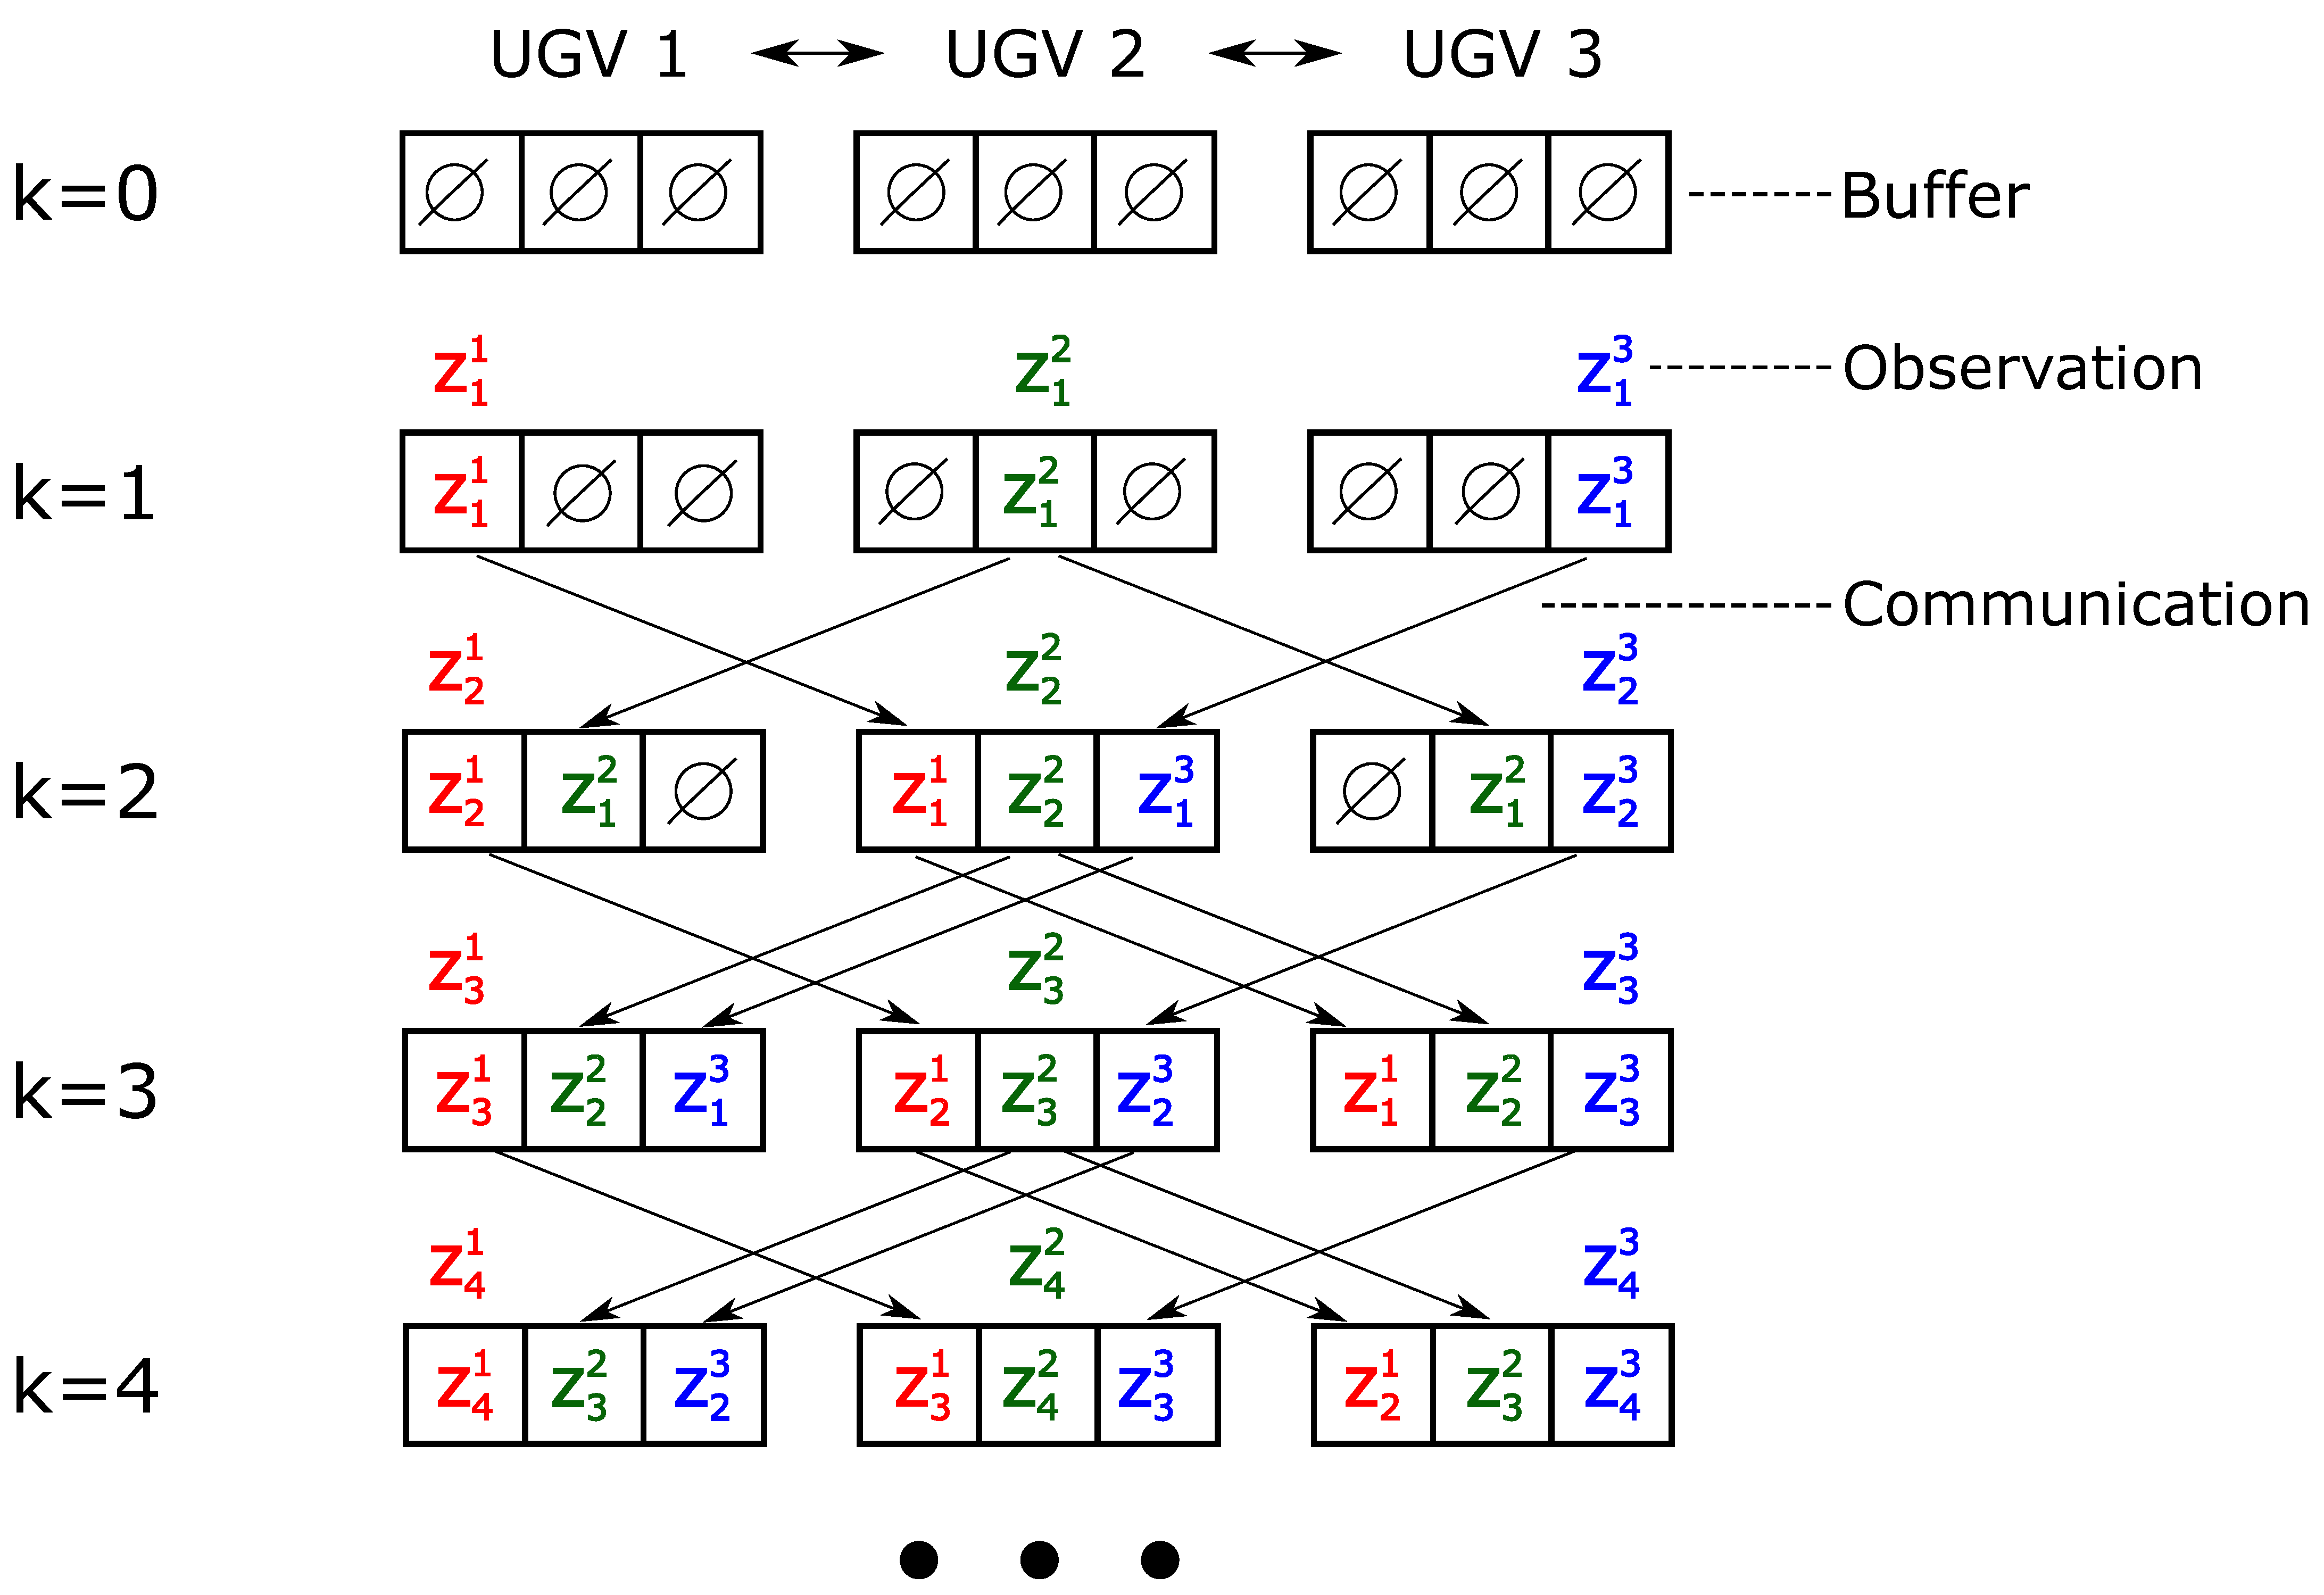
\includegraphics[width=0.49\textwidth]{data_exchange_16-TIE-3798}
		\caption{Example of LIFO with three UGVs using line communication topology. In this case,  $\mathcal{N}_1=\left\lbrace 2 \right\rbrace,\,\mathcal{Q}_1=\left\lbrace 2,3 \right\rbrace;\: \mathcal{N}_2=\left\lbrace 1,3 \right\rbrace,\,\mathcal{Q}_2=\left\lbrace 1,3 \right\rbrace;\: \mathcal{N}_3=\left\lbrace 2 \right\rbrace,\,\mathcal{Q}_3=\left\lbrace 1,2 \right\rbrace$.}
		\label{fig:LIFO}
		\vspace{-1em}
	\end{figure}
	
	\subsection{Algorithm of LIFO-DBF for Static Target}\label{subsec:LIFO-dbf-sta-tar} 
	
	This section derives the LIFO-DBF algorithm for localizing a static target. 
	It is assumed that all UGVs know the sensor model of other UGVs.
	According to \Cref{cor2}, $\mathbf{z}^i_k$ and $\mathbf{z}^{i}_{1:k}$ in \Cref{eqn:bayes_upd} equals $\mathbf{z}^{CB,i}_k$ and $\mathbf{z}^{CB,i}_{1:k}$, respectively.
	The assumption of static target can simplify the Bayesian filter as the prediction step becomes trivial. 
	At time $k$, the $i^\text{th}$ UGV starts from the last-step individual PDF that is locally stored, i.e., $P^i_{pdf}(\X|\mathbf{z}^{i}_{1:k-1})$\footnote{Since the target is static, we drop the subscript $k$ in $\X_k$.}. 
	The $i^\text{th}$ individual PDF is then updated by fusing all measurements in $\mathbf{z}^i_k$:
	\small\begin{align*}\label{eqn:LIFO-dbf-sta-tar}
		P^i_{pdf}(\X|\mathbf{z}^{i}_{1:k})&=K_iP^i_{pdf}(\X|\mathbf{z}^i_{1:k-1})P(\mathbf{z}^i_k|\X)\notag\\
		&=K_iP^i_{pdf}(\X|\mathbf{z}^{i}_{1:k-1})\prod\limits_{j=1}^{N}P(z^j_{k^i_j}|\X),
	\end{align*}\normalsize
	
	where
	\small\begin{equation*}
		K_i=\left[\int\limits_{\X\in S} P^i_{pdf}(\X|\mathbf{z}^{i}_{1:k-1})\prod\limits_{j=1}^{N}P(z^j_{k^i_j}|\X)d\X\right]^{-1}.
	\end{equation*}\normalsize
	
	\subsection{Algorithm of LIFO-DBF for Moving Target}\label{subsec:LIFO-dbf-mov-tar}
	This section derives the LIFO-DBF for localizing a moving target. 
	Instead of storing last-step PDF, at time $k$ each UGV maintains an individual PDF of time $(k-N)$ and a collection of measurement history, called the \textit{record set}, from time $(k-N+1)$ to $k$. 
	The $i^\text{th}$ individual PDF is then alternatively predicted and updated by using the aforementioned Bayesian filter (\Cref{eqn:bayes_pred,eqn:bayes_upd}) from $(k-N)$ to $k$ to obtain $P^i_{pdf}(\X_k|\mathbf{z}^{i}_{1:k})$.
	
	\cref{fig:LIFO-DBF} illustrates the LIFO-DBF procedure for the $1^\text{st}$ UGV as an example \footnote{Due to the space limit, in this figure we use $P^i_{pdf}(k)$, $P^i_{pdf}(k-N)$ and $P^i_{pdf}(k-N+1)$ to represent $P^i_{pdf}(\X|\mathbf{z}^{i}_{1:k})$ $P^i_{pdf}(\X|\mathbf{z}^{i}_{1:k-N})$ and $P^i_{pdf}(\X|\mathbf{z}^{i}_{1:k-N+1})$, respectively.}.
	$\Omega^i_{\xi}\,\left(\xi=1,\dots,N\right) $ denote the index set of UGVs whose measurement at time $(k-N+\xi)$ is stored in $i^\text{th}$ UGV's record set, i.e. $\Omega^i_{\xi}=\left\lbrace j\in \mathcal{Q}_i \bigcup \left\lbrace i \right\rbrace | z^j_{k-N+\xi} \text{ is in the record set} \right\rbrace$.
	The \textbf{LIFO-DBF algorithm} for moving target is stated in \cref{alg:lifo-dbf}.
	
	\begin{figure}%[thpb]
		\centering
		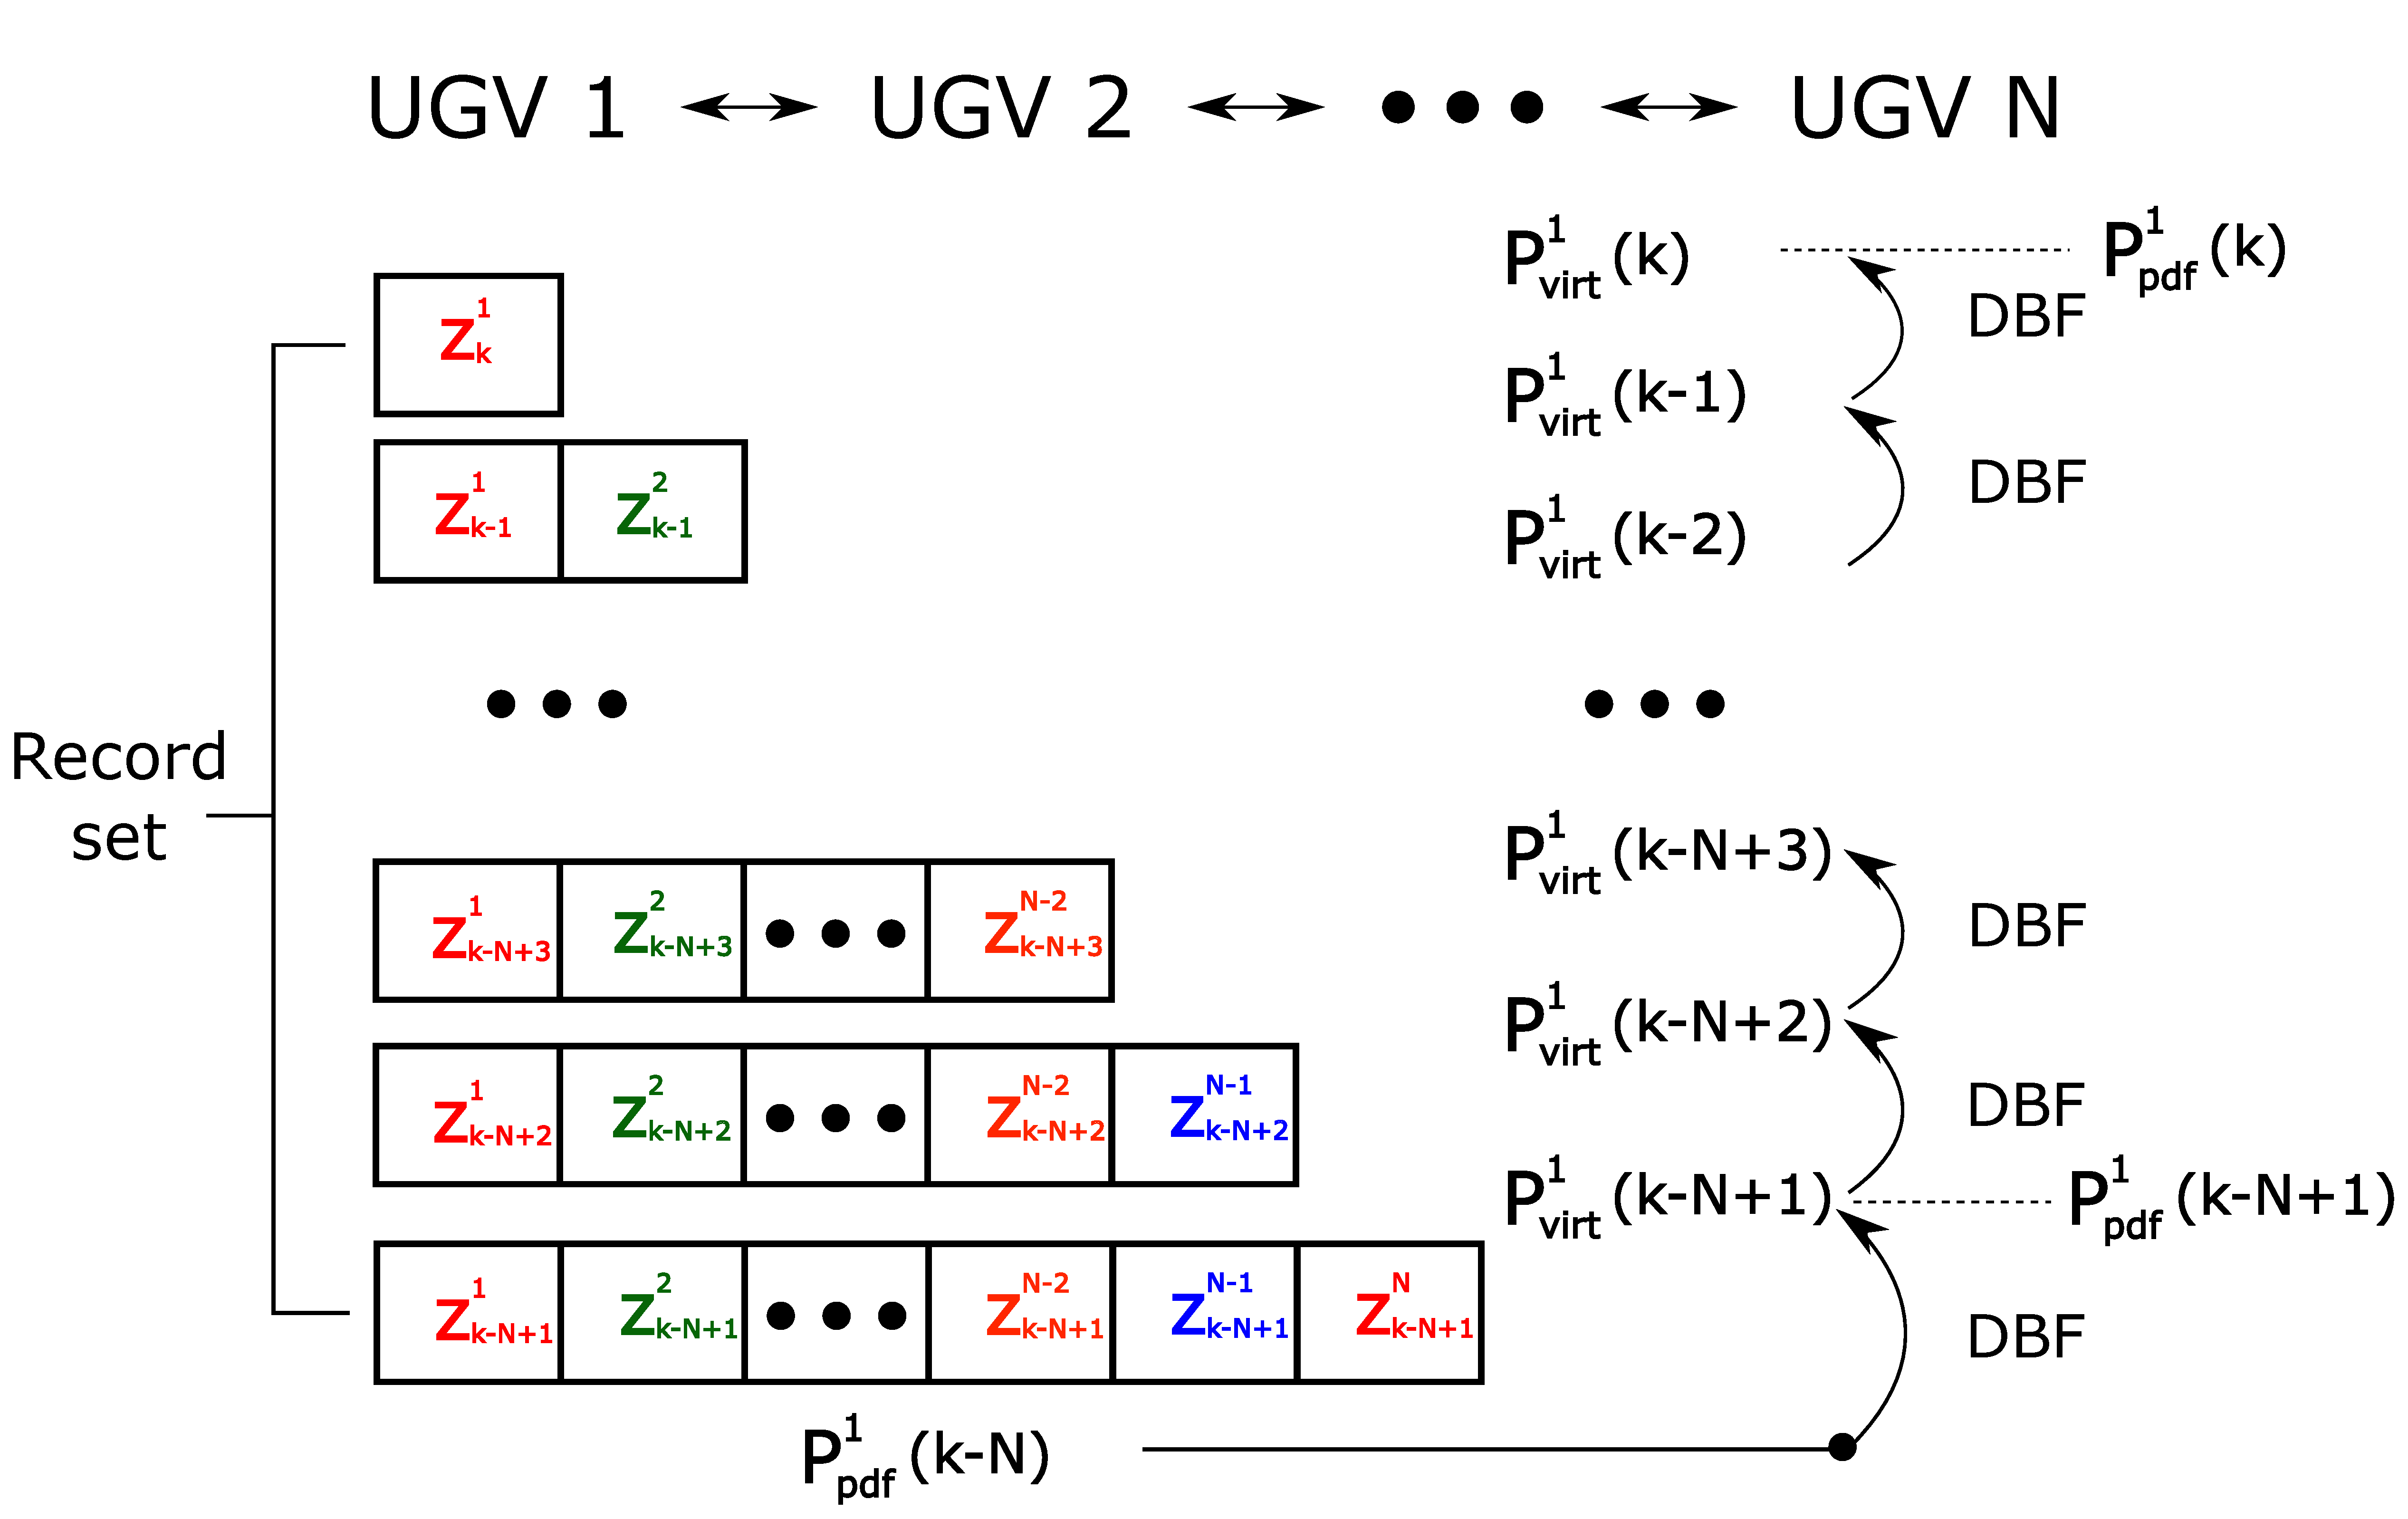
\includegraphics[width=0.51\textwidth]{DBF_demo_16-TIE-3798}
		\caption{Example of LIFO-DBF for $1^\text{st}$ UGV at time $k$. 	 
			Networked UGVs take a line topology. %, shown in the top. 
			The stored individual PDF is represented by $ P^1_{pdf}(k-N)$.
			The UGV first calculates $ P^1_{virt}(k-N+1)$, defined in \Cref{alg:lifo-dbf}, and then stores it as $ P^1_{pdf}(k-N+1)$. 
			Repeating DBF until obtaining $ P^1_{pdf}(k)$.
			In this example, $\Omega^1_{\xi}=\left\lbrace 1,2,\dots,N+1-\xi\right\rbrace $, $\xi=1,\dots,N$.}
		\label{fig:LIFO-DBF}
		\vspace{-1em}
	\end{figure}
	
	%\medskip
	%\begin{rem}
	It is worth noting that, for the static target, each UGV only needs current-step CB to update individual PDFs. 
	Therefore, besides storing its own individual PDF of size $O(M^2)$, only current-step CB of size $O(N)$ is stored in an UGV's memory and all previous CBs can be discarded, which means that the size of needed memory is $O(N+M^2)$. 
	On the contrary, for the moving target, each UGV needs to store a set of measurement history
	%	(except current step CB) triangular matrix
	of size $O(N^2)$ and an individual PDF of size $O(M^2)$. Therefore the size of the needed memory for each UGV is $O(M^2+N^2)$.
	This is generally larger than that of statistics dissemination-based methods, the memory of which is $O(M^2)$. 
	Besides, additional computation power is needed for LIFO-DBF compared to statistics dissemination-based methods.
	Therefore, LIFO-DBF sacrifices storage space and computation resource for reducing communication burden. 
	This is actually desirable for real applications as local memory of vehicles is usually abundant compared to the limited bandwidth for communication.
	%\end{rem}
	
	
	\begin{algorithm}
		\caption{LIFO-DBF Algorithm for Moving Target}\label{alg:lifo-dbf}
		\begin{algorithmic}
			\State For $i^\text{th}$ UGV at $k^\text{th}$ step:
			\State After updating CB by \cref{alg:lifo},	
			%		\State \textbf{(1)} 	
			\State\textbf{(1)} Initialize a \textit{virtual PDF} by assigning the stored individual PDF to it:
			\small\begin{equation*}
				P^i_{virt}(\X_{k-N})= P^i_{stored},
				%			P^i_{pdf}(\X_{k-N}|z^1_{1:k-N},\dots,z^N_{1:k-N}).
			\end{equation*}\normalsize		
			where the stored individual PDF is for time $(k-N)$:
			\small\begin{equation*}
				P^i_{stored} = P^i_{pdf}(\X_{k-N}|z^1_{1:k-N},\dots,z^N_{1:k-N}).
			\end{equation*}\normalsize	
			\State\textbf{(2)} For $\xi=1$ to $N$, iteratively repeat two steps of Bayesian filtering:
			%	\begin{enumerate}
			%		\item 
			
			\State(2.1) Prediction 
			\small\begin{align*}
				&P_{virt}^{pre}(\X_{k-N+\xi})\\=&\int_{S} P(\X_{k-N+\xi}|\X_{k-N+\xi-1})P^i_{virt}(\X_{k-N+\xi-1})d\X_{k-N+\xi-1}.
			\end{align*} \normalsize
			
			%		\item 
			\State(2.2) Updating
			\small\begin{gather*}
				P^i_{virt}(\X_{k-N+\xi})=K_\xi P_{virt}^{pre}(\X_{k-N+\xi})\prod\limits_{j\in\Omega^i_{\xi}}P(z^j_{k-N+\xi}|\X_{k-N+\xi}).\\
				K_\xi=\left[\int_S P_{virt}^{pre}(\X_{k-N+\xi})\prod\limits_{j\in\Omega^i_{\xi}}P(z^j_{k-N+\xi}|\X_{k-N+\xi})d\X_{k-N+\xi}\right]^{-1}.
			\end{gather*} \normalsize
			%	\end{enumerate}
			
			\State(2.3) When $\xi=1$, if $z^j_{k-N+1}\neq\emptyset$ for $\forall j\in \left\lbrace1,\dots,N\right\rbrace$, then the virtual PDF is equivalent to the individual PDF for time $(k-N+1)$. Store it to replace the old PDF:
			\small\begin{equation*}
				P^i_{stored}=P^i_{virt}(\X_{k-N+1}),
			\end{equation*}\normalsize
			where 
			\small\begin{equation*}
				P^i_{virt}(\X_{k-N+1})=P^i_{pdf}(\X_{k-N+1}|z^1_{1:k-N+1},\dots,z^N_{1:k-N+1}).
			\end{equation*}\normalsize
			
			\State\textbf{(3)} Individual PDF of $i^\text{th}$ UGV at time $k$ is
			$P^i_{pdf}(\X_{k}|\mathbf{z}^{i}_{1:k})=P^i_{virt}(\X_k)$.		
		\end{algorithmic}
	\end{algorithm}
	
	\section{Proof of Consistency}\label{sec:consist_proof} %and Consensus
	This section proves the consistency of the maximum a posteriori (MAP) estimator of LIFO-DBF under unbiased sensors (sensors without offset).
	An estimator of a state is said to be consistent if it converges in probability to the true value of the state \cite{amemiya1985advanced}.
	Consistency is an important metric for stochastic filtering approaches \cite{chen2003bayesian} and it differs from the concept of consensus; consensus implies that the estimation results of all sensors converge to a same value, while consistency not only implies achieving consensus asymptotically, but also requires that the estimated value converge to the true value. 
	
	We first prove the consistency for static UGVs.
	The consistency for moving UGVs is subsequently proved.
	For simplicity and clarity, we assume $S$ is a finite set (e.g. a finely discretized field) and the
	target motion is relatively slow compared to the filtering dynamics. 
	
	\subsection{Static UGVs}
	The consistency of LIFO-DBF for static UGVs is stated as follows: 
	\begin{thm}\label{thm:LIFO-dbf-sta-tar}
		Assume the UGVs are static and the sensors are unbiased, then the MAP estimator of target position converges in probability to the true position of the target using LIFO-DBF, i.e.,
		\small\begin{equation*}
			\lim\limits_{k\rightarrow \infty}
			P(\X^{i,MAP}_k=\xg)=
			1,\;i=1,\dots,N,
		\end{equation*}\normalsize
		where 
		\small\begin{equation*}
			\X^{i,MAP}_k=\arg\max\limits_{\X}P^i_{pdf}(\X|\mathbf{z}^{i}_{1:k}).
		\end{equation*}
	\end{thm}
	
	\begin{proof}
		First we look at the asymptotic behavior of $P^i_{pdf}(\X|\mathbf{z}^{i}_{1:k})$.
		The batch form of DBF at $k^\text{th}$ step is:
		\small\begin{subequations}\label{eqn:bayes_batch}
			\begin{align}
				P^i_{pdf}(\X|\mathbf{z}^{i}_{1:k})&=P^i_{pdf}(\X|z^1_{1:k^i_1},\dots,z^N_{1:k^i_N})\\
				&=\frac{P^i_{pdf}(\X)\prod\limits_{j=1}^{N}\prod\limits_{l=1}^{k^i_j}P(z^j_l|\X)}{\sum\limits_{\X\in S}P^i_{pdf}(\X)\prod\limits_{j=1}^{N}\prod\limits_{l=1}^{k^i_j}P(z^j_l|\X)}\label{eqn:bayes_batch2}.
			\end{align}
		\end{subequations}\normalsize 
		The decomposition into multiplication in \Cref{eqn:bayes_batch2} results from the conditional independence of measurements given $\X$.
		
		
		Comparing the conditional probability of an arbitrary position $x\in S$ with that of target position $\xg$:
		\small\begin{equation}\label{eqn:cmp}
			\frac{P^i_{pdf}(\X=x|\mathbf{z}^{i}_{1:k})}{P^i_{pdf}(\X=\xg|\mathbf{z}^{i}_{1:k})}=\frac{P^i_{pdf}(x)\prod\limits_{j=1}^{N}\prod\limits_{l=1}^{k^i_j}P(z^j_l|x)}{P^i_{pdf}(\xg)\prod\limits_{j=1}^{N}\prod\limits_{l=1}^{k^i_j}P(z^j_l|\xg)}.\footnote{For the purpose of simplicity, we abbreviate $P^i_{pdf}(\X=x)$ and $P(z^j_l|\X=x)$ as $P^i_{pdf}(x)$ and $P(z^j_l|x)$ in this proof.}
		\end{equation}\normalsize
		
		Take the logarithm of \Cref{eqn:cmp} and average it over $k$ steps:
		\small\begin{equation}\label{eqn:cmp_log}
			\frac{1}{k}\ln\frac{P^i_{pdf}(\X=x|\mathbf{z}^{i}_{1:k})}{P^i_{pdf}(\X=\xg|\mathbf{z}^{i}_{1:k})}=\frac{1}{k}\ln\frac{P^i_{pdf}(x)}{P^i_{pdf}(\xg)}+\sum\limits_{j=1}^{N}\frac{1}{k}\sum\limits_{l=1}^{k^i_j}\ln\frac{P(z^j_l|x)}{P(z^j_l|\xg)}.
		\end{equation}\normalsize
		
		Since $P^i_{pdf}(x)$ and $P^i_{pdf}(\xg)$ are bounded and $P^i_{pdf}(\X)$ is initialized such that $P^i_{pdf}(\xg)\neq 0$, then
		\small\begin{equation*}\label{eqn:cmp_lim1}
			\lim\limits_{k\rightarrow \infty}\frac{1}{k}\ln\frac{P^i_{pdf}(x)}{P^i_{pdf}(\xg)}= 0.
		\end{equation*}\normalsize
		
		Utilizing the facts: (1) $z^j_l$ are conditionally independent samples from $P(z^j_l|\xg)$ and (2) $k-N<k^i_j\leq k$, the law of large numbers yields
		\small\begin{subequations}\label{eqn:cmp_lim2}
			\begin{align} 
				\frac{1}{k}\sum\limits_{l=1}^{k^i_j}\ln\frac{P(z^j_l|x)}{P(z^j_l|\xg)}&\overset{P}{\longrightarrow}\mathbb{E}_{z^j_l} \left[\ln\frac{P(z^j_l|x)}{P(z^j_l|\xg)}\right]\\
				&=\int_{z^j_l} P(z^j_l|\xg)\ln\frac{P(z^j_l|x)}{P(z^j_l|\xg)} dz^j_l\\
				&=-D_{KL}\left(P(z^j_l|\xg)\|P(z^j_l|x)\right),
			\end{align}
		\end{subequations}\normalsize
		where ``$\overset{P}{\longrightarrow}$" represents ``convergence in probability'' and $D_{KL}(P_1\|P_2)$ denotes the Kullback-Leibler (KL) divergence between two probability distributions $P_1$ and $P_2$.
		The KL divergence has the property \cite{mackay2003information} that $\forall P_1,\,P_2$,
		\begin{equation*}
			D_{KL}(P_1\|P_2)\leq 0, \text{ equality holds iff } \; P_1=P_2.
		\end{equation*}
		This leads to the following results:
		
		\begin{equation*}
			\lim\limits_{k\rightarrow \infty}\frac{1}{k}\sum\limits_{l=1}^{k^i_j}\ln\frac{P(z^j_l|x)}{P(z^j_l|\xg)}\;
			\begin{cases}
				<0,&\quad \text{if}\; x\neq \xg\\
				=0,&\quad \text{if}\; x= \xg
			\end{cases}.
		\end{equation*}
		
		Then by considering the limit of \Cref{eqn:cmp_log} when $k\rightarrow\infty$, we get:
		
		\begin{equation}\label{subeqn:limit}
			\lim\limits_{k\rightarrow \infty}\frac{1}{k}\ln\frac{P^i_{pdf}(x|\mathbf{z}^{i}_{1:k})}{P^i_{pdf}(\xg|\mathbf{z}^{i}_{1:k})}\;
			\begin{cases}
				<0,&\quad \text{if}\; x\neq \xg\\
				=0,&\quad \text{if}\; x= \xg
			\end{cases}.
		\end{equation}
		
		\Cref{subeqn:limit} implies that
		
		\begin{equation*}
			\frac{P^i_{pdf}(x|\mathbf{z}^{i}_{1:k})}{P^i_{pdf}(\xg|\mathbf{z}^{i}_{1:k})}\overset{P}{\longrightarrow}
			\begin{cases}
				0,&\quad \text{if}\; x\neq \xg\\
				1,&\quad \text{if}\; x= \xg
			\end{cases}.
		\end{equation*}
		
		Therefore,
		\small\begin{equation*}
			\lim\limits_{k\rightarrow \infty}
			P_{pdf}^i(\X=\xg|\mathbf{z}^{i}_{1:k})=1.
		\end{equation*}\normalsize
		Thus
		\small\begin{equation*}
			\lim\limits_{k\rightarrow \infty}
			P(\X^{i,MAP}_k=\xg)=1.
		\end{equation*}\normalsize
	\end{proof}	
	
	\subsection{Moving UGVs}
	This subsection considers the case of using moving UGVs to localize a target.
	The difficulty of consistency proof for this case lies in the fact that each UGV makes measurements at multiple positions.
	Here, the main idea of the proof is to classify UGV measurement positions into two disjoint sets: \textit{infinite-measurement spots} that contain positions where a UGV visits infinitely many times as time tends to infinity, and \textit{finite-measurement spots} that contain positions where the UGV visits finitely many times (i.e., the UGV does not visit again after a finite time period).
	Before stating the main theorem, the following lemma is introduced.
	\begin{lem}\label{lem1}
		For a set of UGVs moving within a collection of finite positions, each UGV has at least one position where infinite measurements are made as $k$ tends to infinity.
	\end{lem}
	
	\begin{proof}
		Let $n^{i,k}_s$ denote the times that $i^\text{th}$ UGV visits $s^\text{th}$ position up to time $k$. Then, $\sum\limits_{s\in S} n^{i,k}_s=k$. It is straightforward to see that $\exists n^{i,k}_s,$ such that $n^{i,k}_s\rightarrow \infty,$ as $k\rightarrow \infty$.
	\end{proof}
	\medskip
	
	\begin{thm}\label{thm:LIFO-dbf-mov-sen}
		Assume UGVs move within a collection of finite positions and sensors are unbiased, then the MAP estimator of target position converges in probability to the true position of the target using LIFO-DBF, i.e.,
		\small\begin{equation*}
			\lim\limits_{k\rightarrow \infty}
			P(\X^{i,MAP}_k=\xg_k)=1,\;i=1,\dots,N.
		\end{equation*}\normalsize
	\end{thm}
	
	\begin{proof}
		According to \Cref{thm:LIFO-dbf-sta-tar}, the batch form of DBF at $k^\text{th}$ step is
		\small\begin{equation}\label{eqn:cmp2}
			\frac{P^i_{pdf}(\X=x|\mathbf{z}^i_{1:k})}{P^i_{pdf}(\X=\xg|\mathbf{z}^i_{1:k})}=\frac{P^i_{pdf}(x)\prod\limits_{j=1}^{N}\prod\limits_{l=1}^{k^i_j}P(z^j_l|x;x^j_l)}{P^i_{pdf}(\xg)\prod\limits_{j=1}^{N}\prod\limits_{l=1}^{k^i_j}P(z^j_l|\xg;x^j_l)}.
		\end{equation}\normalsize
		
		The only difference from \Cref{eqn:cmp} is that $P(z^j_l|x;x^j_l)$ in \Cref{eqn:cmp2} varies as the UGV moves. 
		For each UGV, there exists at least one position where infinite measurements are made as $k\rightarrow \infty$, according to \Cref{lem1}. 
		For the finite-measurement spots, by referring to \Cref{eqn:cmp_lim2}, it is easy to know that their contribution to \Cref{eqn:cmp_log} diminishes when $k\rightarrow \infty$.
		Therefore, proof using \Cref{eqn:cmp2} can be reduced to only considering infinite-measurement spots and the rest of proof is similar to that of \Cref{thm:LIFO-dbf-sta-tar}.
	\end{proof}
	
	\begin{rem}
		The assumption of unbiased sensors are important for the consistency of the estimator. In fact, with unknown non-zero bias, the distribution of $z^j_l$ differs from $P(z^j_l|\xg)$, which invalidates the derivation in \Cref{eqn:cmp_lim2} and the consistency proof. 
		This assumption also makes intuitive sense.
		In the extreme case, if each sensor has a very large unknown measurement offset, then the estimated target position of each sensor (without communicating with other sensors) will be very different from each other's.
		Therefore, no common target position can be correctly obtained when they fuse measurements.
	\end{rem}
	\medskip
	
	
	\section{Simulation for Target Localization}\label{sec:sim}
	
	\begin{figure}%[thpb]
		\centering
		\begin{subfigure}[b]{0.21\textwidth}
			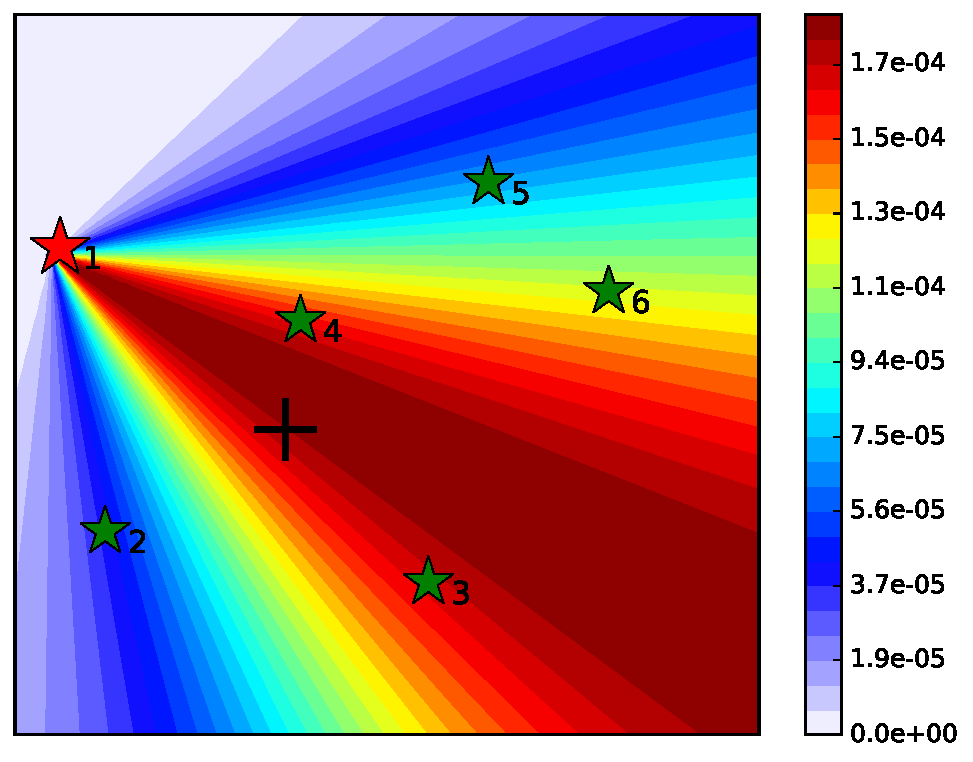
\includegraphics[width=\textwidth]{brg_sta_sen_sta_tar_rbt1_step1_16-TIE-3798}
			\caption{Step 1}\label{fig:sta_sen_sta_tar_sing1}
		\end{subfigure}
		\begin{subfigure}[b]{0.21\textwidth}
			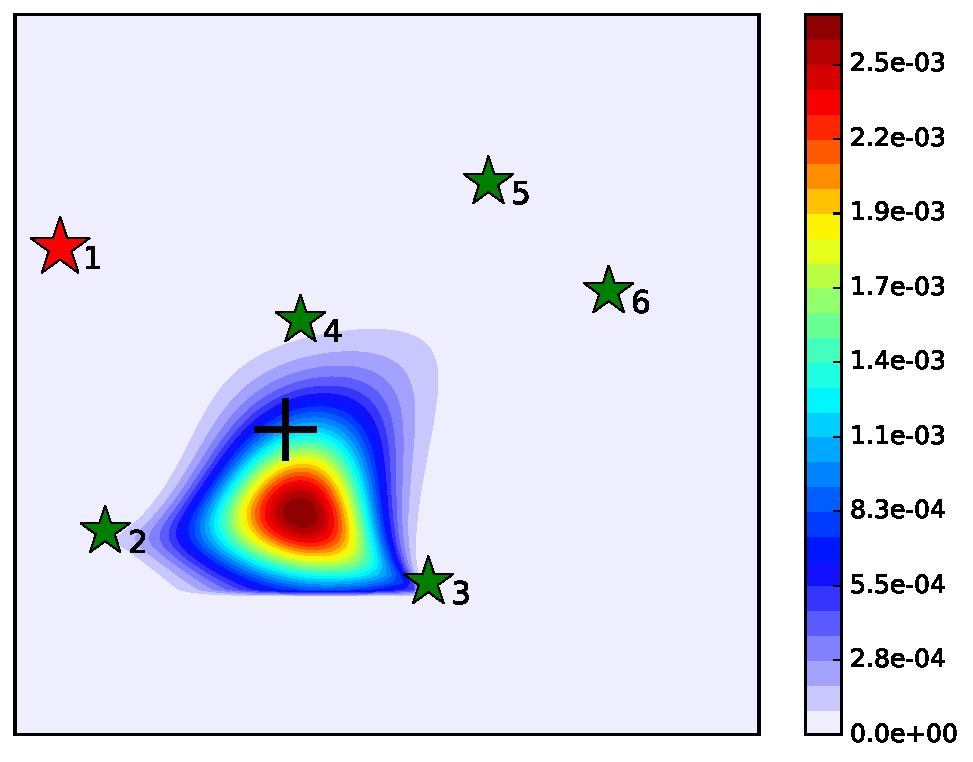
\includegraphics[width=\textwidth]{brg_sta_sen_sta_tar_rbt1_step3_16-TIE-3798}
			\caption{Step 3}\label{fig:sta_sen_sta_tar_sing2}
		\end{subfigure}
		\begin{subfigure}[b]{0.21\textwidth}
			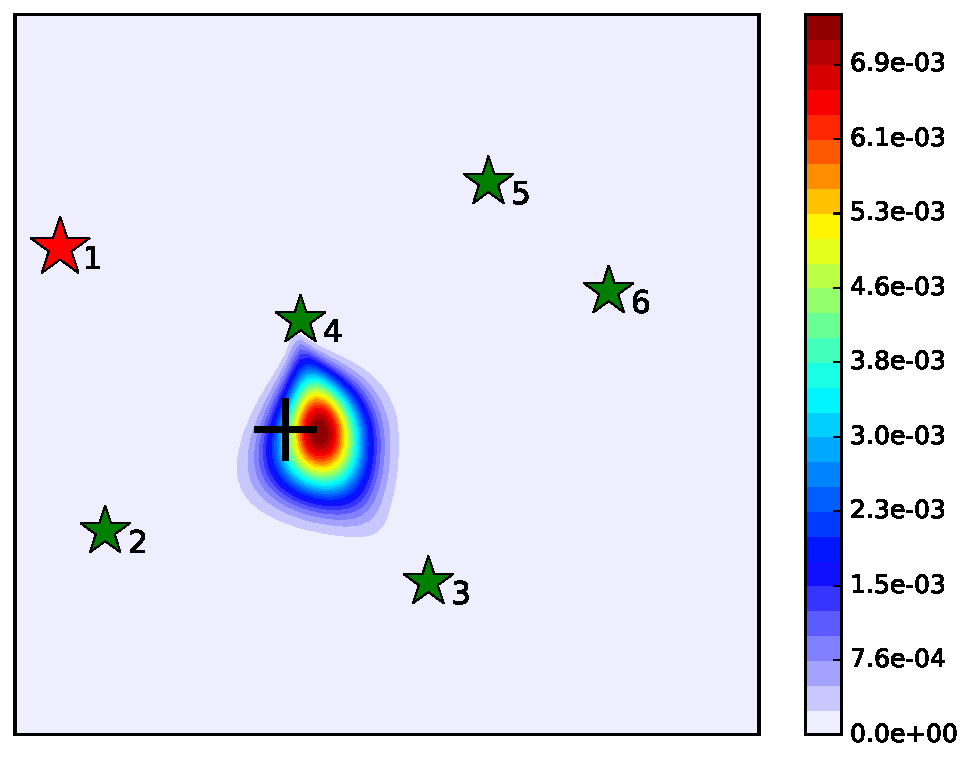
\includegraphics[width=\textwidth]{brg_sta_sen_sta_tar_rbt1_step5_16-TIE-3798}
			\caption{Step 5}\label{fig:sta_sen_sta_tar_sing3}
		\end{subfigure}
		\begin{subfigure}[b]{0.21\textwidth}
			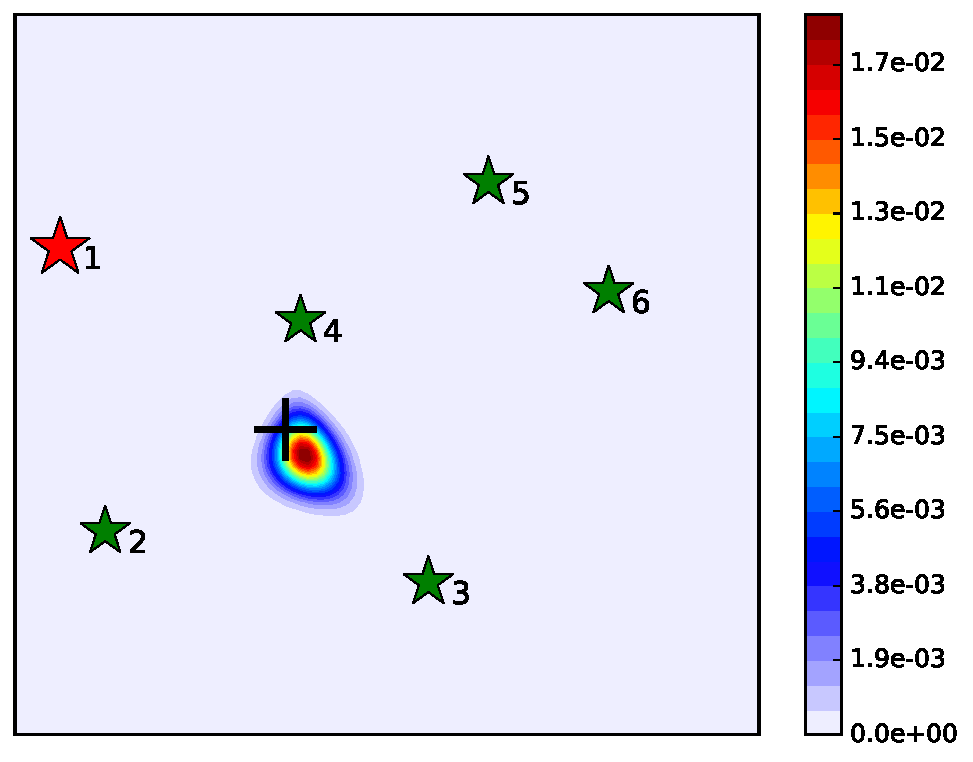
\includegraphics[width=\textwidth]{brg_sta_sen_sta_tar_rbt1_step10_16-TIE-3798}
			\caption{Step 10}\label{fig:sta_sen_sta_tar_sing4}
		\end{subfigure}
		\begin{subfigure}[b]{0.21\textwidth}
			%		\includegraphics[width=\textwidth]{figures/test}
			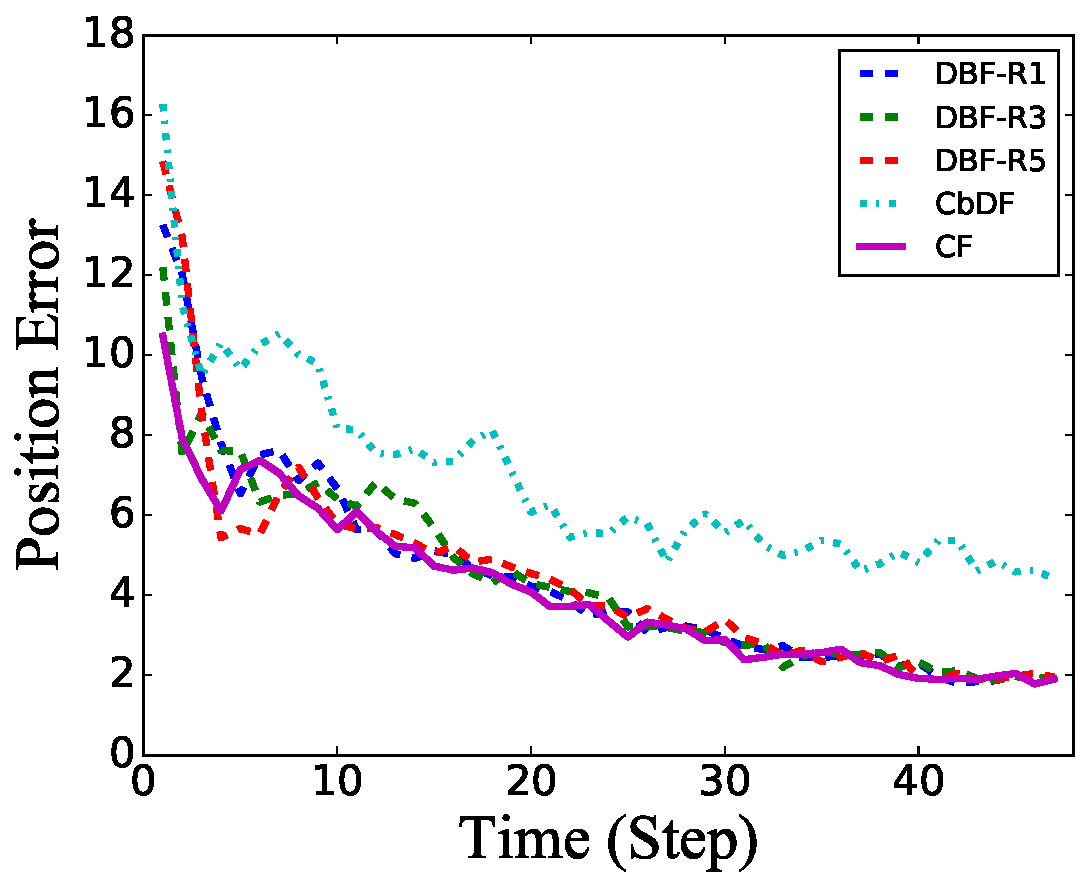
\includegraphics[width=\textwidth]{brg_sta_sen_sta_tar_pos_err_16-TIE-3798}
			\caption{Position Error}\label{fig:sta_sen_sta_tar_pos_err}
		\end{subfigure}
		\begin{subfigure}[b]{0.21\textwidth}
			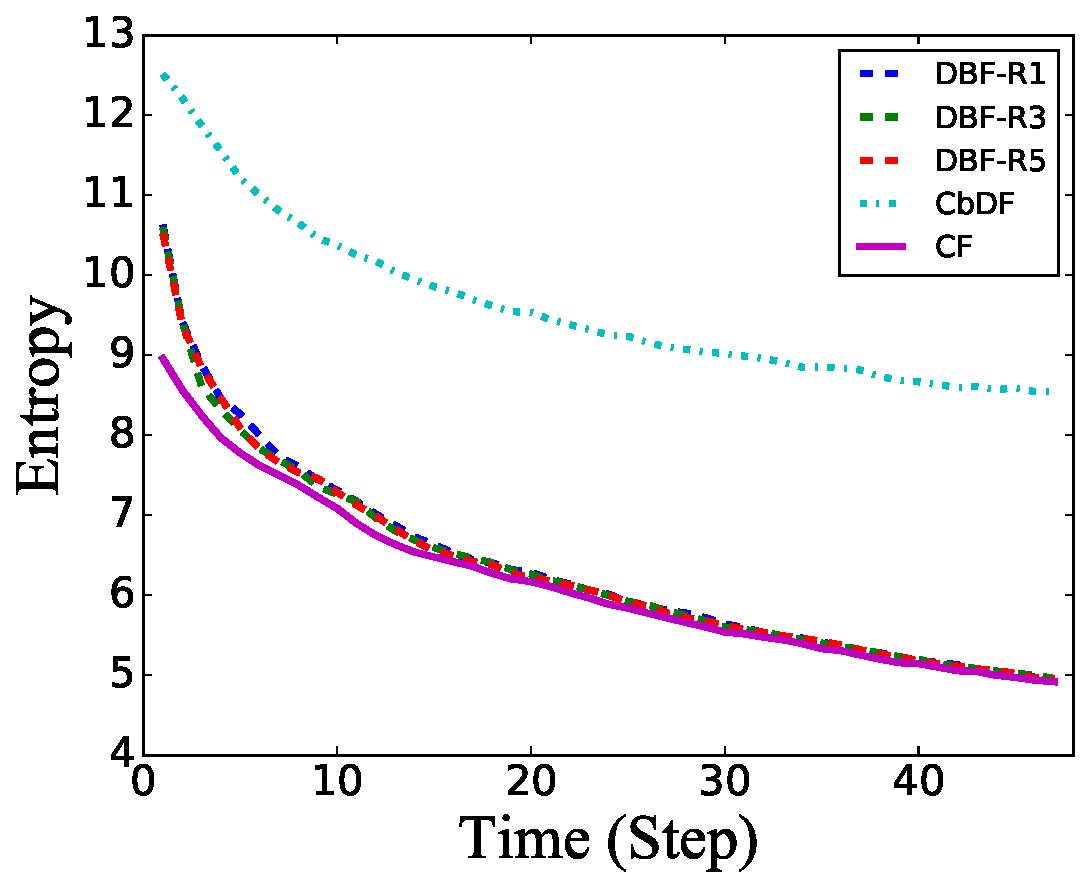
\includegraphics[width=\textwidth]		{brg_sta_sen_sta_tar_entropy_16-TIE-3798}%{figures/test2}
			\caption{Entropy of Individual PDF}\label{fig:sta_sen_sta_tar_entropy}
		\end{subfigure}
		\caption{(a)-(d) The $1^\text{st}$ UGV's individual PDF at different times. 
			The cross stands for the target. Note that the value of the color bar varies among different figures. (e) Average position estimation error of the $1^\text{st}$, $3^\text{rd}$ and $5^\text{th}$ UGV's LIFO-DBF, the CbDF and the CF. (f) Average entropy of individual PDFs.}
		\label{fig:sta_sen_sta_tar}
		\vspace{-1em}
	\end{figure}
	
	\begin{figure}%[thpb]
		\centering
		\begin{subfigure}[b]{0.21\textwidth}
			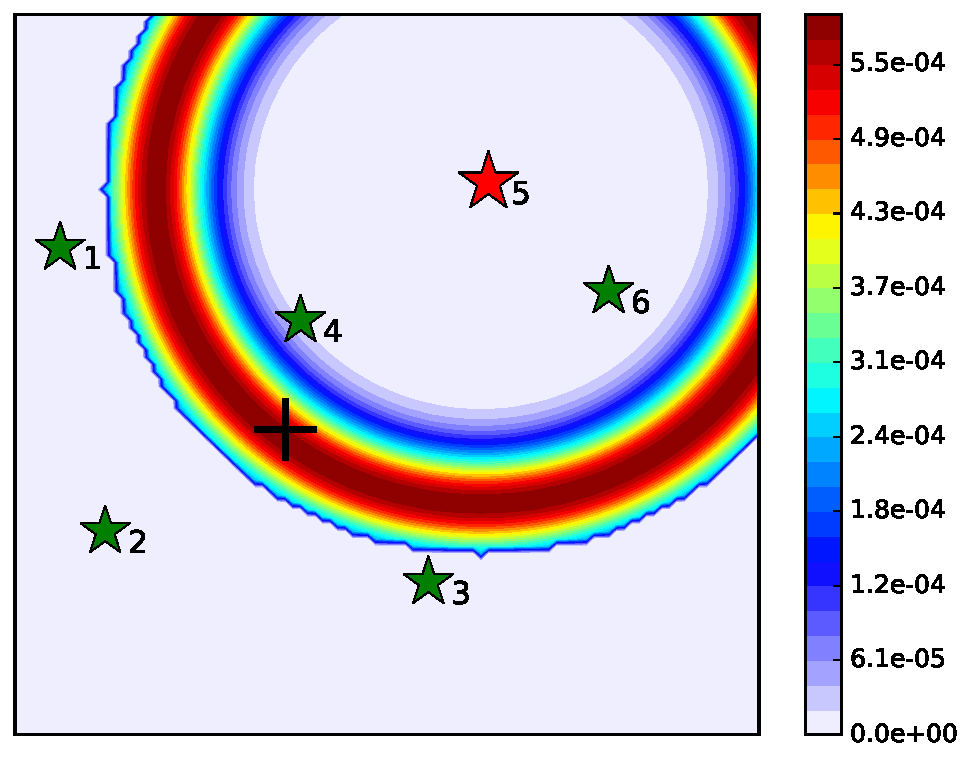
\includegraphics[width=\textwidth]{hetero_sta_sen_sta_tar_rbt5_step1_16-TIE-3798}
			\caption{Step 1}\label{fig:htr_sta_sen_sta_tar_sing1}
		\end{subfigure}
		\begin{subfigure}[b]{0.21\textwidth}
			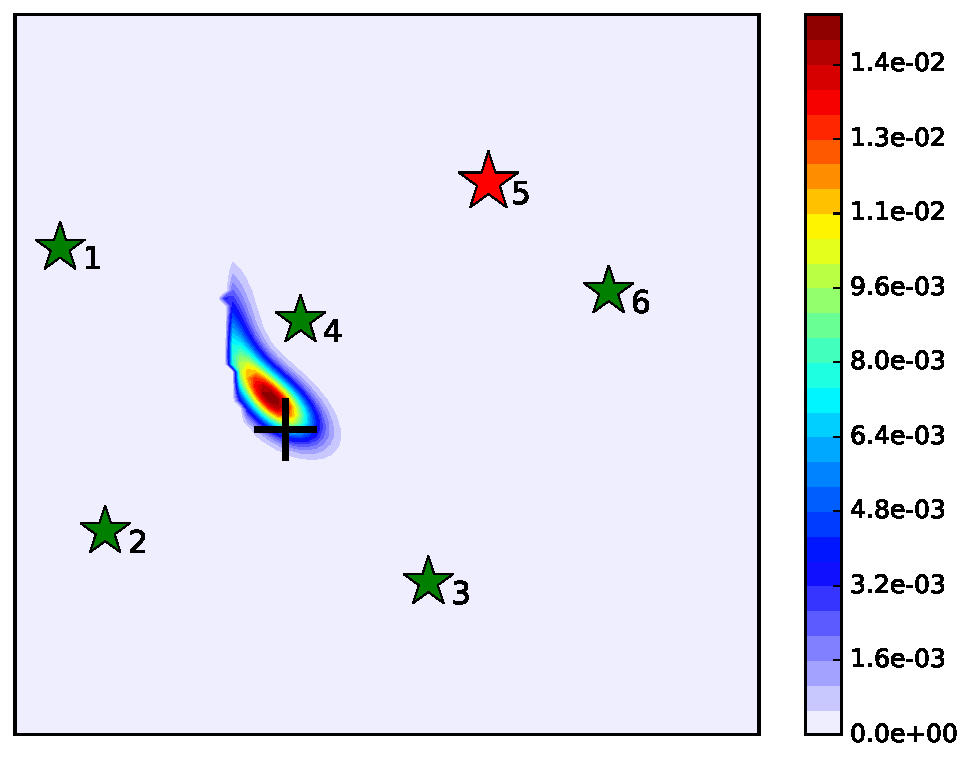
\includegraphics[width=\textwidth]{hetero_sta_sen_sta_tar_rbt5_step3_16-TIE-3798}
			\caption{Step 3}\label{fig:htr_sta_sen_sta_tar_sing2}
		\end{subfigure}
		\begin{subfigure}[b]{0.21\textwidth}
			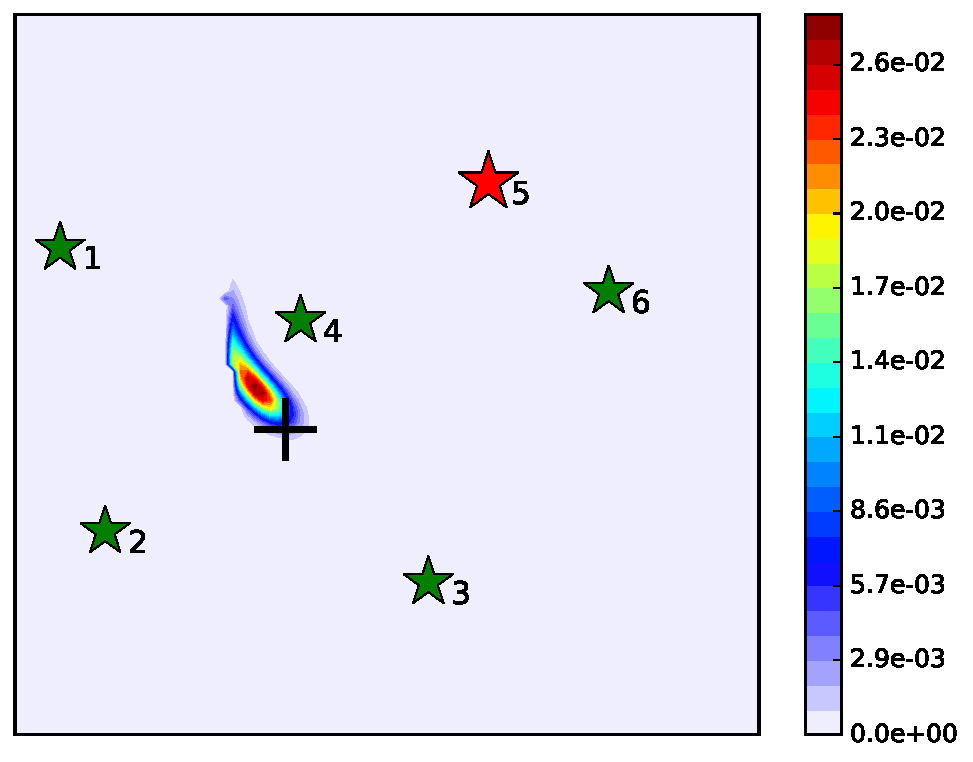
\includegraphics[width=\textwidth]{hetero_sta_sen_sta_tar_rbt5_step5_16-TIE-3798}
			\caption{Step 5}\label{fig:htr_sta_sen_sta_tar_sing3}
		\end{subfigure}
		\begin{subfigure}[b]{0.21\textwidth}
			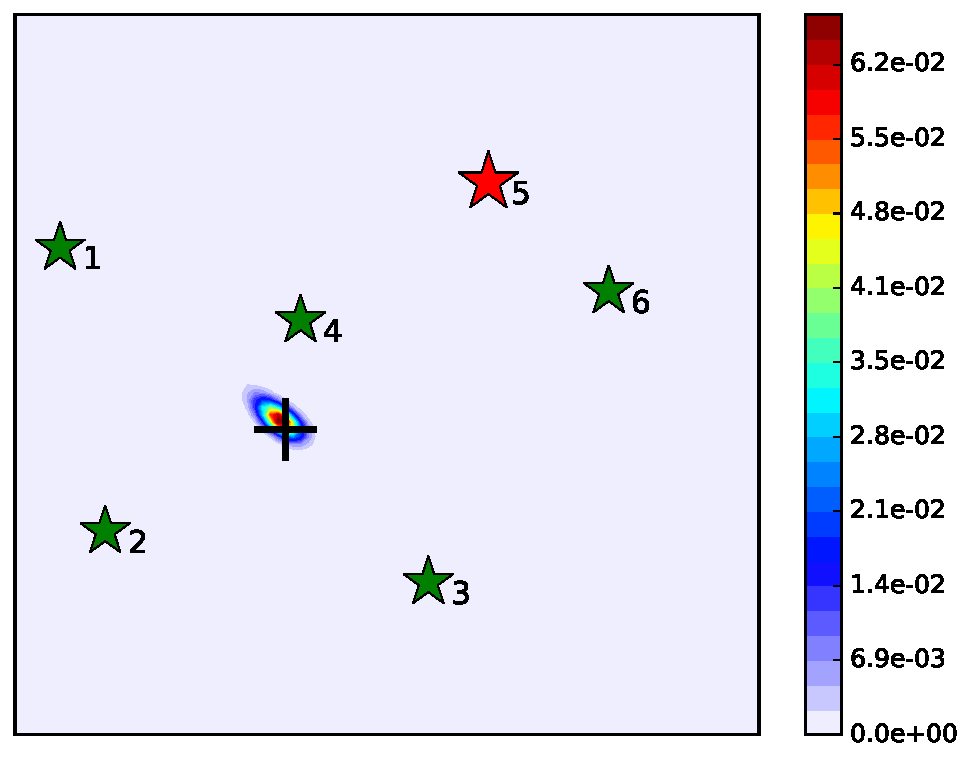
\includegraphics[width=\textwidth]{hetero_sta_sen_sta_tar_rbt5_step10_16-TIE-3798}
			\caption{Step 10}\label{fig:htr_sta_sen_sta_tar_sing4}
		\end{subfigure}
		\begin{subfigure}[b]{0.21\textwidth}
			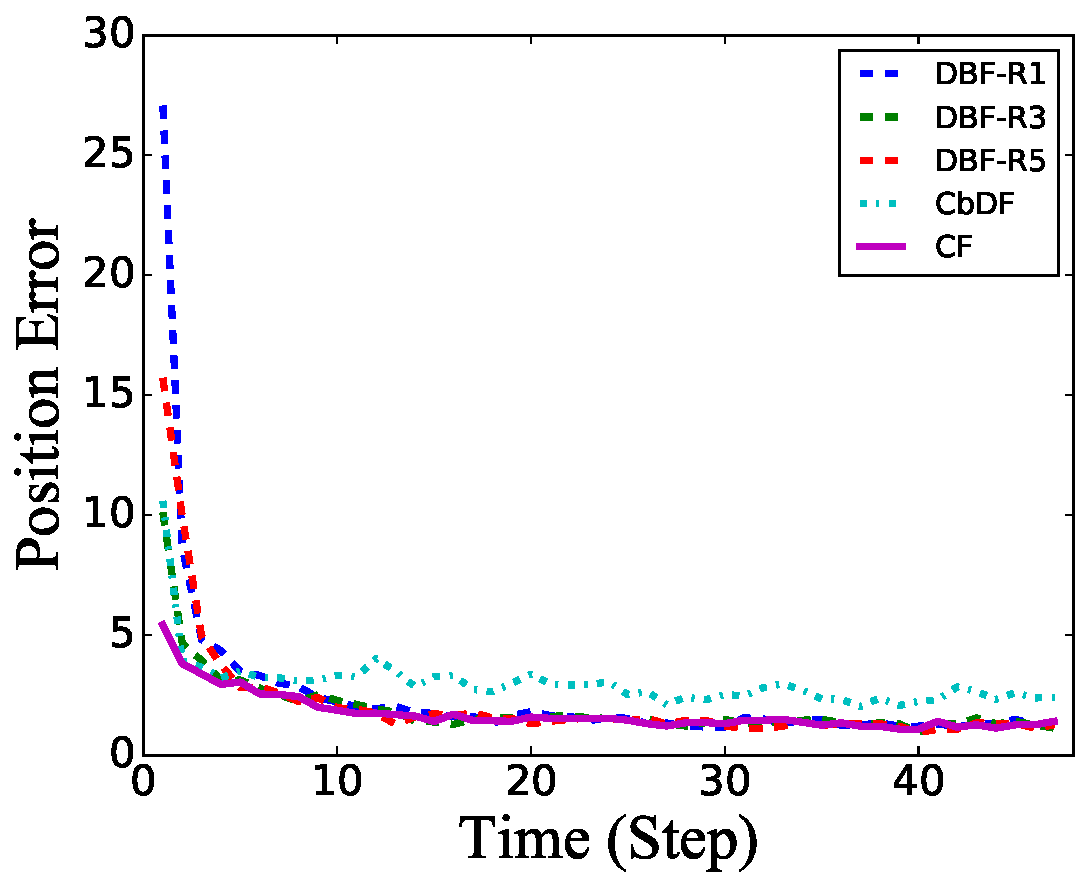
\includegraphics[width=\textwidth]{hetero_sta_sen_sta_tar_pos_err_16-TIE-3798}
			\caption{Position Error}\label{fig:htr_sta_sen_sta_tar_pos_err}
		\end{subfigure}
		\begin{subfigure}[b]{0.21\textwidth}
			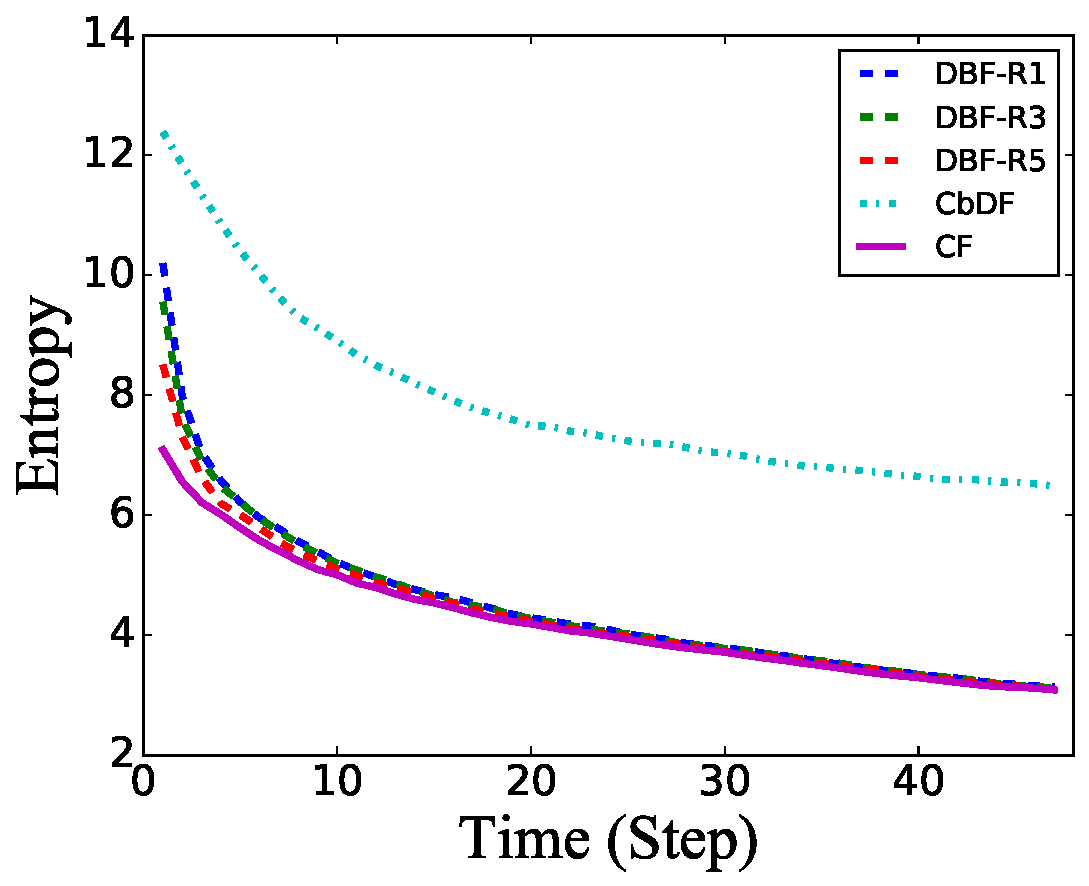
\includegraphics[width=\textwidth]{hetero_sta_sen_sta_tar_entropy_16-TIE-3798}
			\caption{Entropy of Individual PDF}\label{fig:htr_sta_sen_sta_tar_entropy}
		\end{subfigure}
		\caption{(a)-(d) The $5^\text{th}$ UGV's individual PDF at different times. (e) Average position estimation error. (f) Average entropy of individual PDFs.}
		\label{fig:htr_sta_sen_sta_tar}
		\vspace{-1em}
	\end{figure}
	
	
%	\begin{figure}%[thpb]
%		\centering
%		\begin{subfigure}[b]{0.21\textwidth}
%			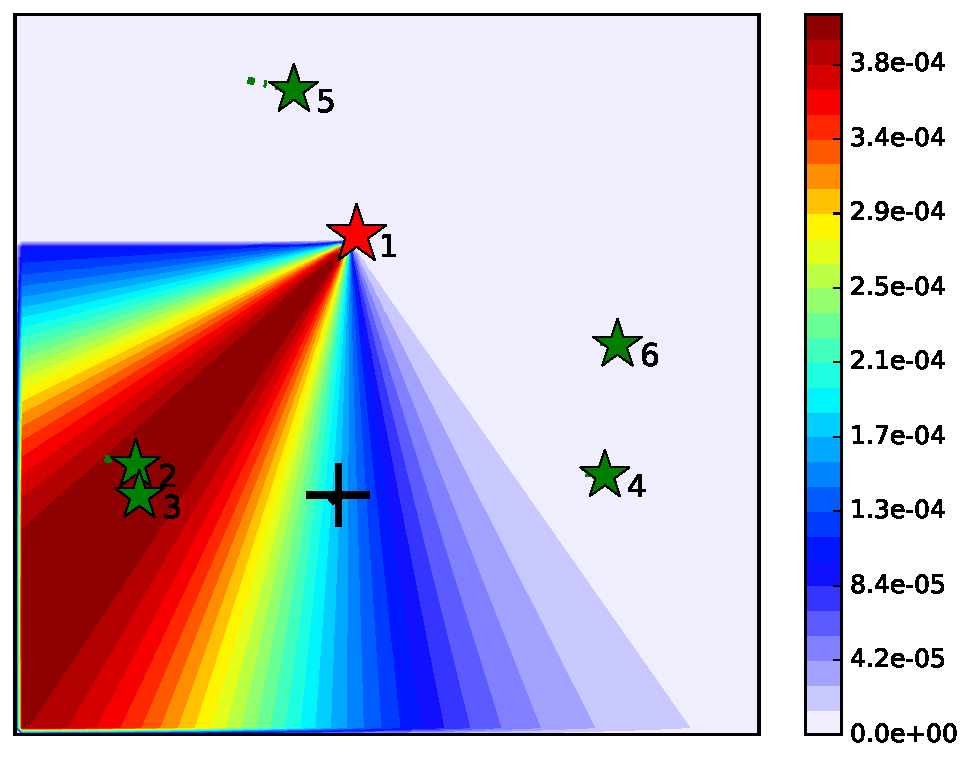
\includegraphics[width=\textwidth]{figures/brg_mov_sen_mov_tar_rbt1_step1}
%			\caption{Step 1}\label{fig:mov_sen_mov_tar_sing1}
%		\end{subfigure}
%		\begin{subfigure}[b]{0.21\textwidth}
%			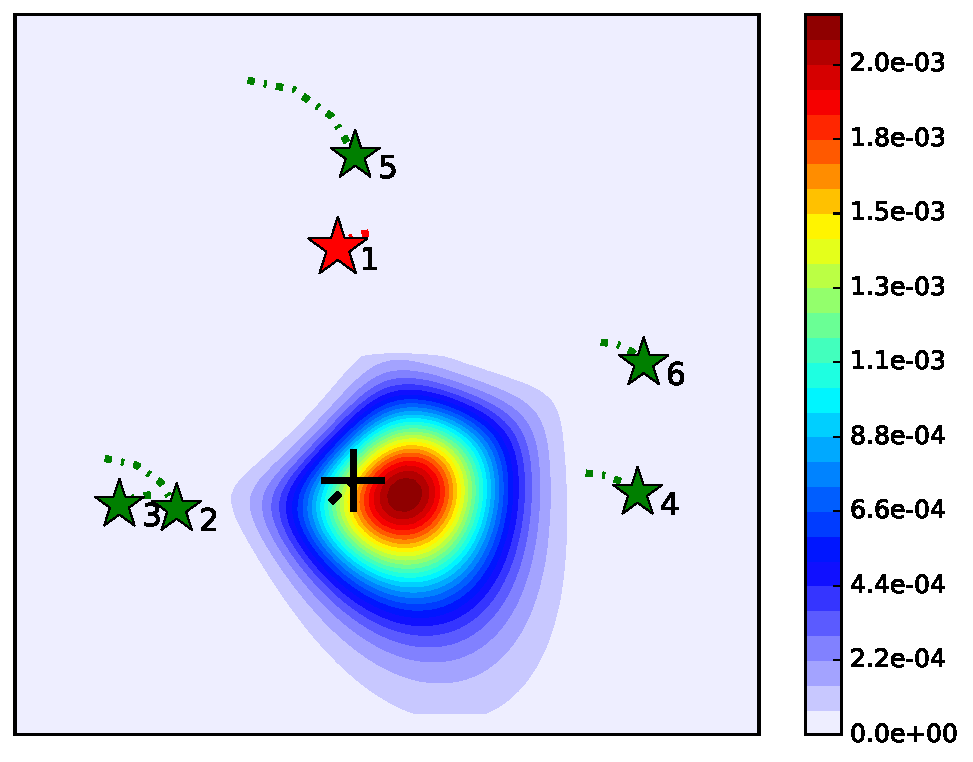
\includegraphics[width=\textwidth]{figures/brg_mov_sen_mov_tar_rbt1_step3}
%			\caption{Step 3}\label{fig:mov_sen_mov_tar_sing2}
%		\end{subfigure}	
%		\begin{subfigure}[b]{0.21\textwidth}
%			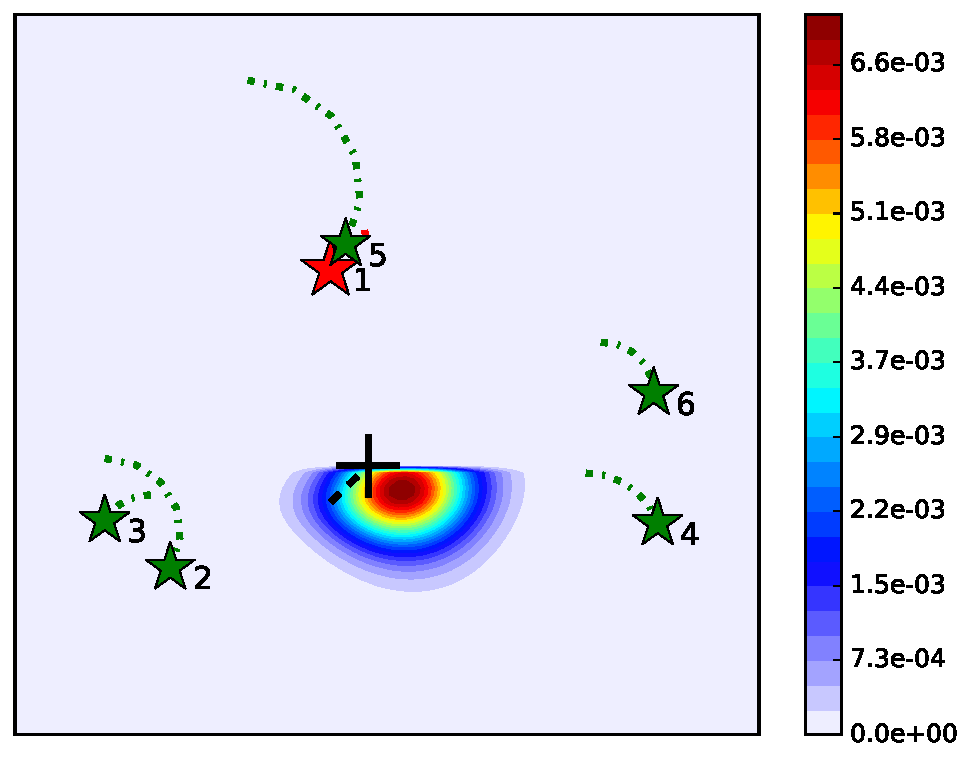
\includegraphics[width=\textwidth]{figures/brg_mov_sen_mov_tar_rbt1_step5}
%			\caption{Step 5}\label{fig:mov_sen_mov_tar_sing3}
%		\end{subfigure}	
%		\begin{subfigure}[b]{0.21\textwidth}
%			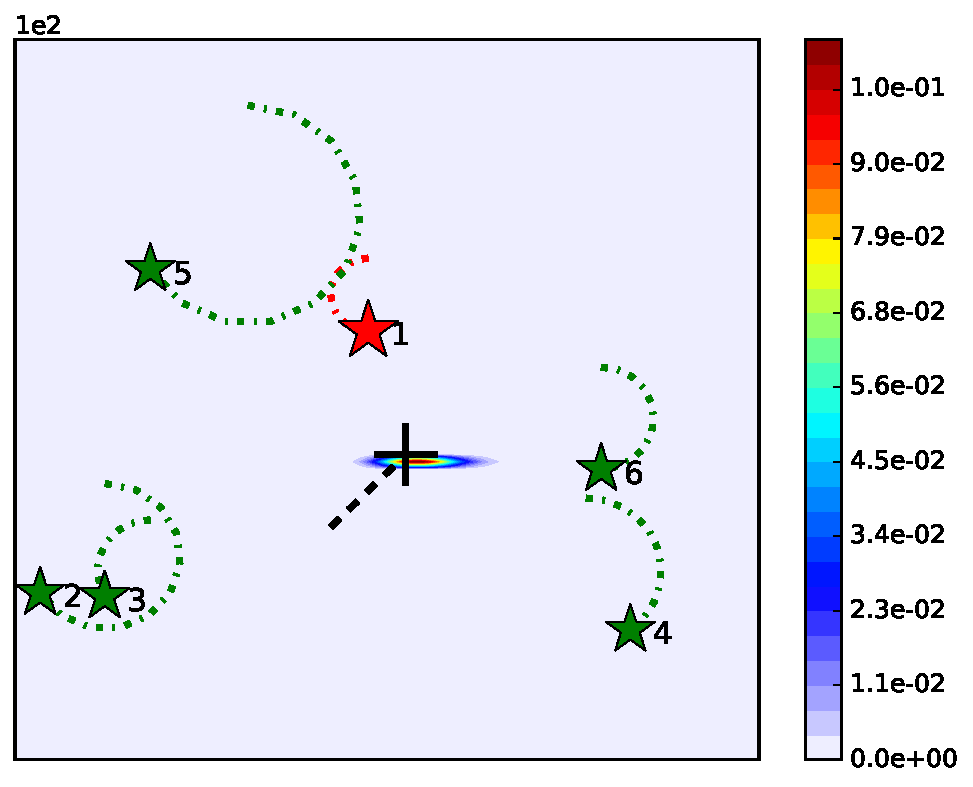
\includegraphics[width=\textwidth]{figures/brg_mov_sen_mov_tar_rbt1_step10}
%			\caption{Step 10}\label{fig:mov_sen_mov_tar_sing4}
%		\end{subfigure}
%		\begin{subfigure}[b]{0.21\textwidth}
%			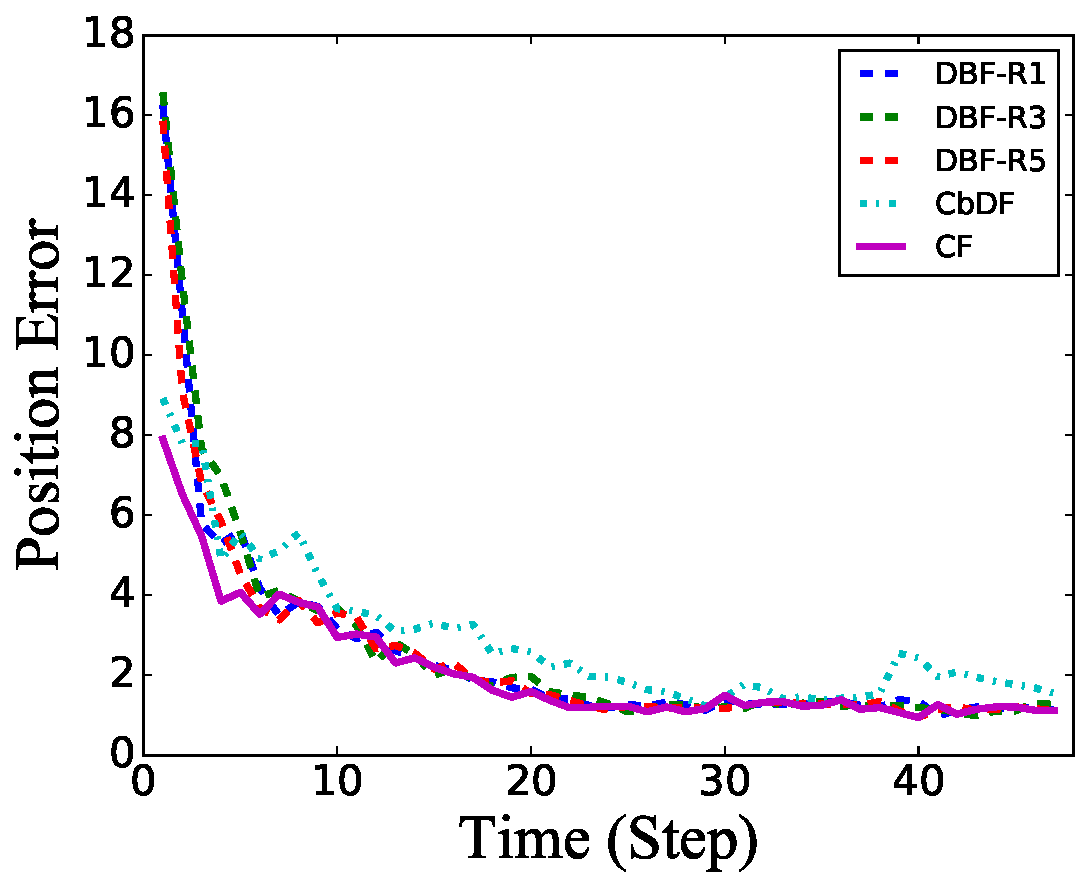
\includegraphics[width=\textwidth]{figures/brg_mov_sen_mov_tar_pos_err.pdf}
%			\caption{Position Error}\label{fig:mov_sen_mov_tar_pos_err}
%		\end{subfigure}
%		\begin{subfigure}[b]{0.21\textwidth}
%			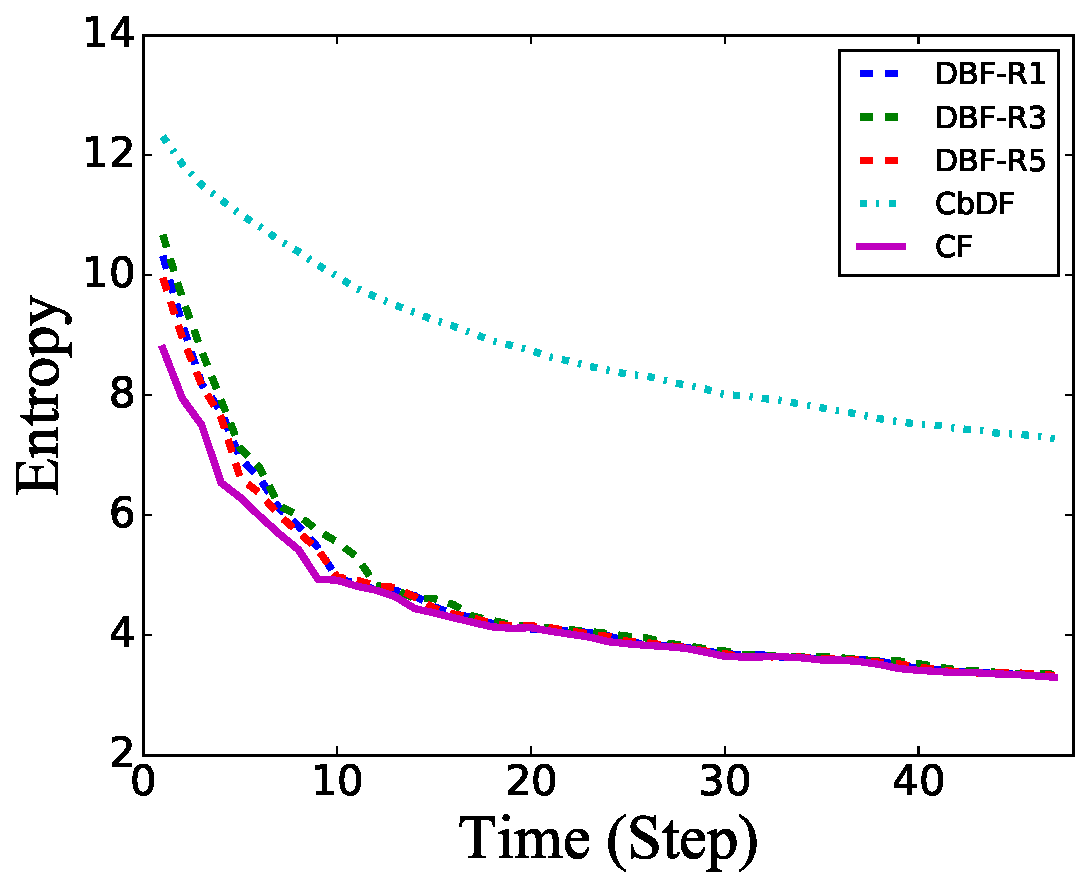
\includegraphics[width=\textwidth]{figures/brg_mov_sen_mov_tar_entropy.pdf}
%			\caption{Entropy of Individual PDF}\label{fig:mov_sen_mov_tar_entropy}
%		\end{subfigure}
%		\caption{(a)-(d) The $1^\text{st}$ UGV's individual PDFs at different times. The green dashed lines represent robots' trajectories. (e) Average position estimation error. (f) Average entropy of individual PDFs.}
%		\label{fig:mov_sen_mov_tar}
%		\vspace{-1.1em}
%	\end{figure}
	
	
	
	Simulation has been conducted to evaluate the effectiveness of LIFO-DBF for target localization using a team of six UGVs.
	The networked UGVs take a ring communication topology that each UGV can communicate with two fixed neighbors.
	DBF is implemented using the histogram filter method, by which the continuous space is finely discretized into finitely many regions and the individual PDF is approximated by the cumulative probability of each region \cite{thrun2005probabilistic}.
	Two types of scenarios are used: in the first scenario, both UGVs and the target are static;
	the second scenario subsequently deals with moving UGVs for localizing a moving target. 
	In the first scenario, we test two different kinds of UGV team: the first UGV team, called the homogeneous team, is equipped with bearing-only sensors; in the second team, called the heterogeneous team, three UGVs are equipped with bearing-only sensor and the other three equipped with range-only sensors.
	In the second scenario, the heterogeneous team is tested.
	The bearing-only sensors are assumed to have large enough sensing range to cover the simulation field and the measurement noise is a zero-mean Gaussian white noise with standard deviation being $0.5$.
	The range-only sensors are assumed to have $360\degree$ field of view and the measurement noise is a zero-mean Gaussian white noise with standard deviation being $5$.
	
	In both scenarios, LIFO-DBF is compared with two commonly adopted approaches in multi-agent filtering: the consensus-based distributed filtering (CbDF) method \cite{olfati2006belief} and the centralized filtering (CF) method \cite{veeravalli2012distributed}.
	The CbDF requires UGVs to continually exchange their individual PDFs with direct neighbors, computing the average of its own and the received PDFs. 
	Multiple rounds of communication and averaging are conducted during the ``Sending Step'' and ``Receiving Step'' in \Cref{alg:lifo} at each step to ensure the convergence of UGV's individual PDFs.
	The CF assumes a central unit that can constantly receive and fuse all UGVs' latest measurements into a single PDF.
	Ten test trials with randomly generated initial UGV and target positions are run and each trial is terminated after 50 time steps.
	The average error between the estimated (using the MAP estimator) and true target position and the average entropy of individual PDFs of all 10 trials using these three approaches are compared.
	
	\begin{figure}%[thpb]
		\centering
		\begin{subfigure}[b]{0.21\textwidth}
			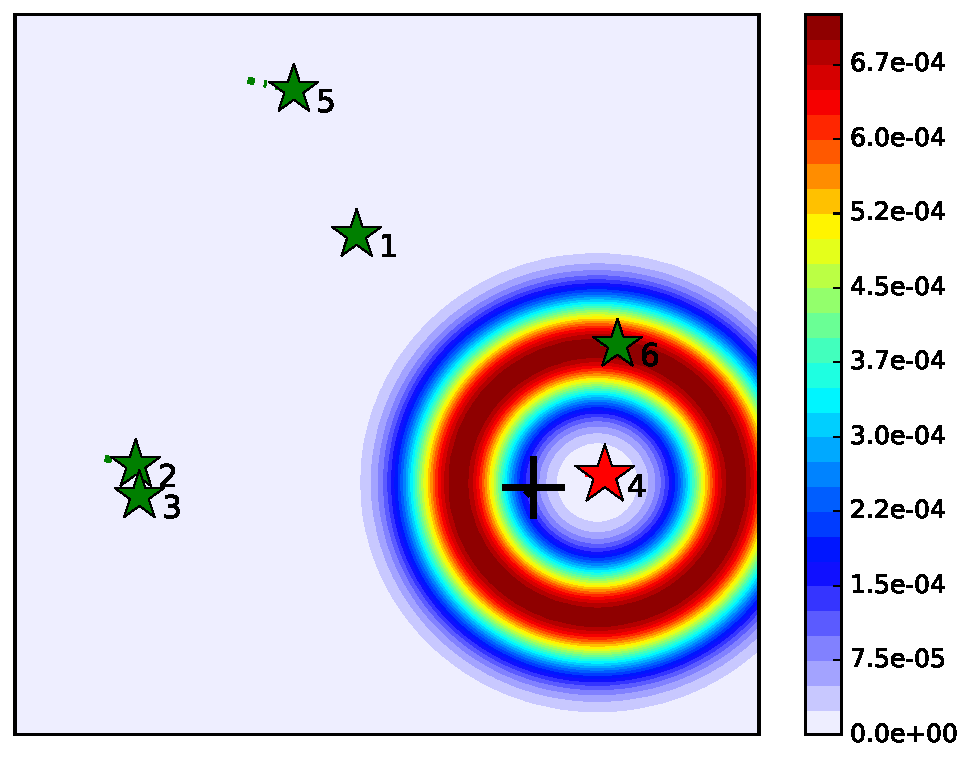
\includegraphics[width=\textwidth]{hetero_mov_sen_mov_tar_rbt4_step1_16-TIE-3798}
			\caption{Step 1}\label{fig:htr_mov_sen_mov_tar_sing1}
		\end{subfigure}
		\begin{subfigure}[b]{0.21\textwidth}
			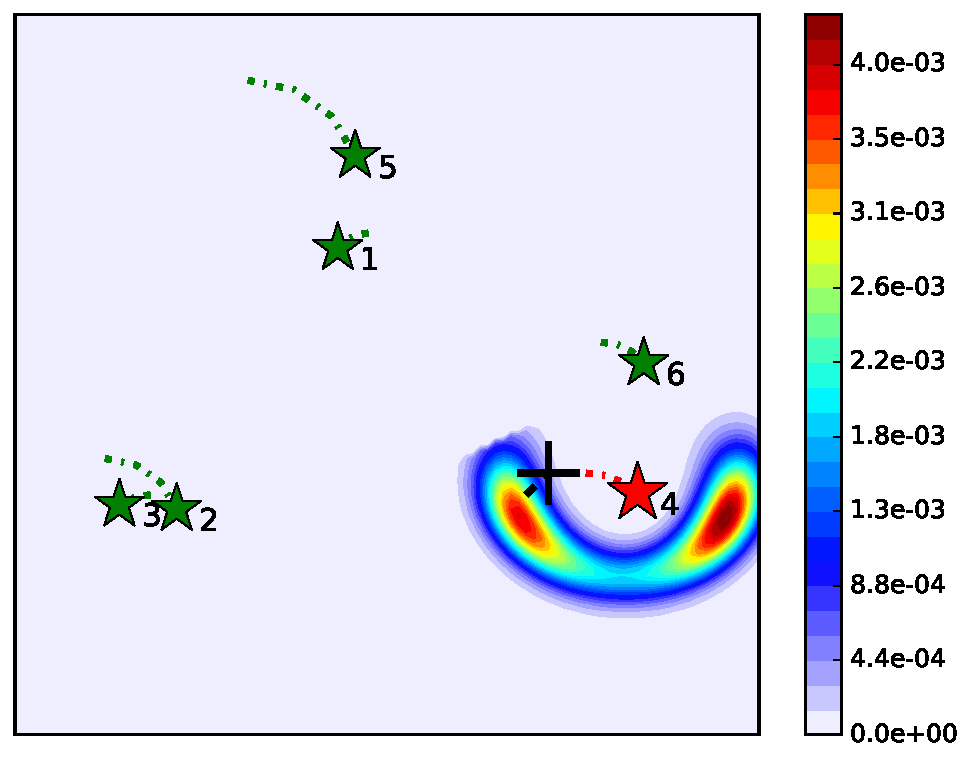
\includegraphics[width=\textwidth]{hetero_mov_sen_mov_tar_rbt4_step3_16-TIE-3798}
			\caption{Step 3}\label{fig:htr_mov_sen_mov_tar_sing2}
		\end{subfigure}
		\begin{subfigure}[b]{0.21\textwidth}
			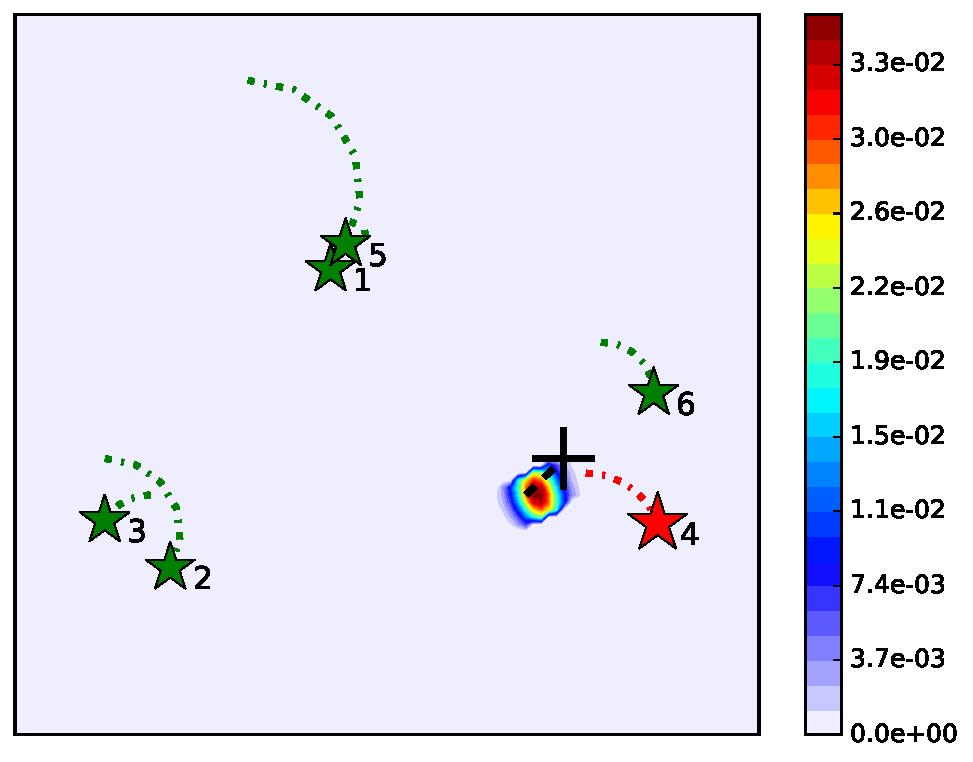
\includegraphics[width=\textwidth]{hetero_mov_sen_mov_tar_rbt4_step5_16-TIE-3798}
			\caption{Step 5}\label{fig:htr_mov_sen_mov_tar_sing3}
		\end{subfigure}
		\begin{subfigure}[b]{0.21\textwidth}
			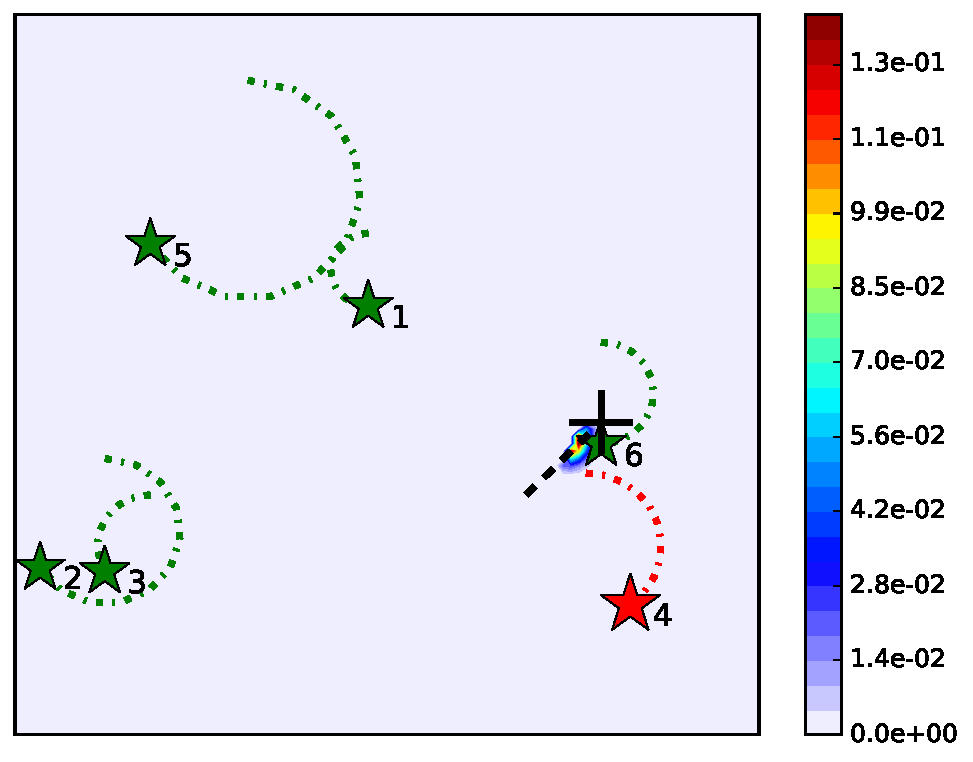
\includegraphics[width=\textwidth]{hetero_mov_sen_mov_tar_rbt4_step10_16-TIE-3798}
			\caption{Step 10}\label{fig:htr_mov_sen_mov_tar_sing4}
		\end{subfigure}
		\begin{subfigure}[b]{0.21\textwidth}
			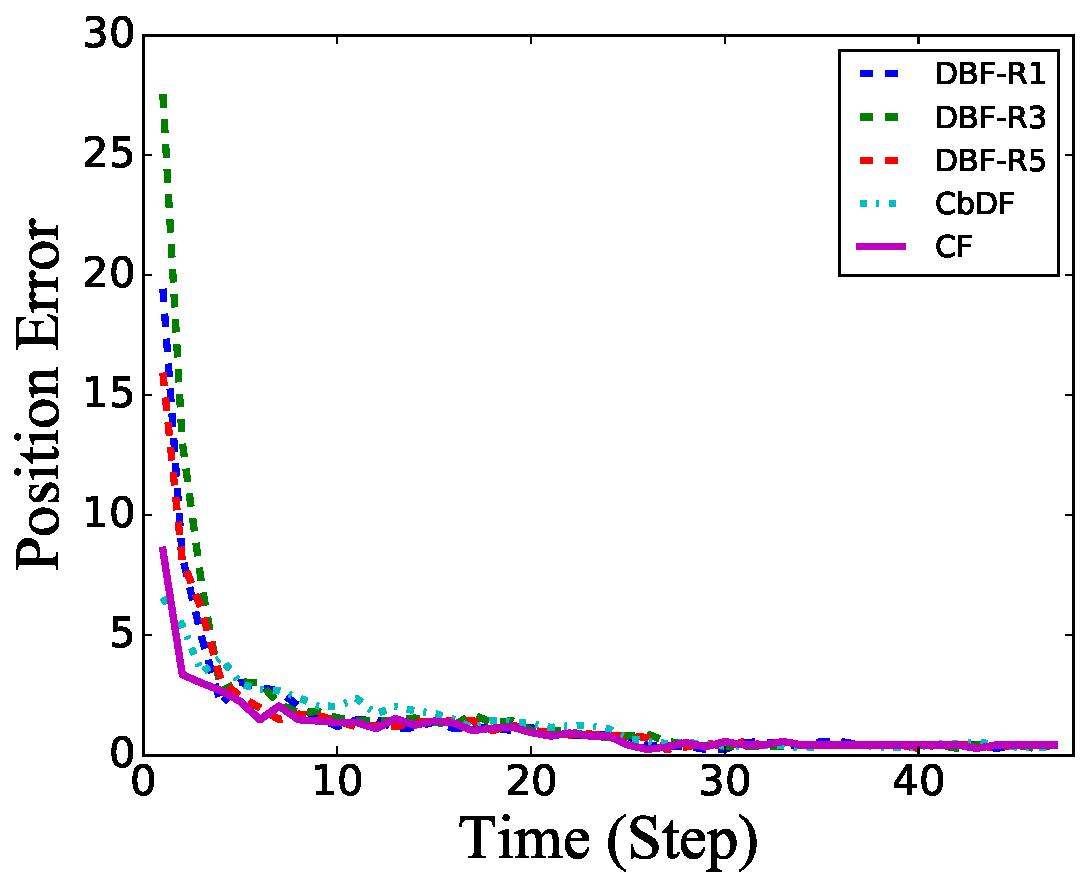
\includegraphics[width=\textwidth]{hetero_mov_sen_mov_tar_pos_err_16-TIE-3798}
			\caption{Position Error}\label{fig:htr_mov_sen_mov_tar_pos_err}
		\end{subfigure}
		\begin{subfigure}[b]{0.21\textwidth}
			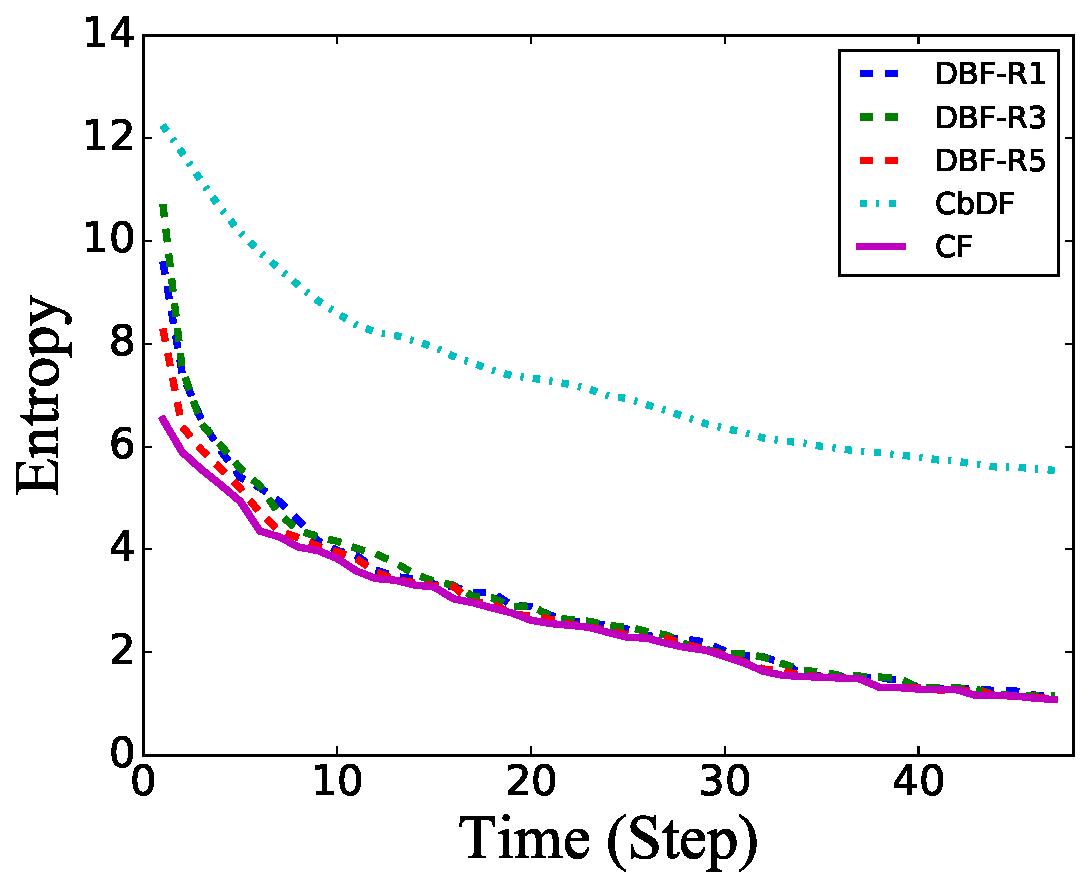
\includegraphics[width=\textwidth]{hetero_mov_sen_mov_tar_entropy_16-TIE-3798}
			\caption{Entropy of Individual PDF}\label{fig:htr_mov_sen_mov_tar_entropy}
		\end{subfigure}
		\caption{(a)-(d) The $4^\text{th}$ UGV's individual PDF at different times. (e) Average position estimation error. (f) Average entropy of individual PDFs.}
		%\label{fig:sta_sen_sta_tar}
		\vspace{-1.2em}
	\end{figure}
	
	\subsection{Static UGVs, Static Target}
	The individual PDF of each UGV is initialized as a uniform distribution over a bounded space. 
	At each time step, each UGV executes the LIFO-DBF for static target (\Cref{subsec:LIFO-dbf-sta-tar}) to update their estimation of target position.
	The evolution of the $1^\text{st}$ robot's individual PDF is shown in \cref{fig:sta_sen_sta_tar_sing1,fig:sta_sen_sta_tar_sing2,fig:sta_sen_sta_tar_sing3,fig:sta_sen_sta_tar_sing4}. 
	Since the robot is equipped with a noisy bearing-only sensor, the measurement at step $1$ results in a wide distribution with the peak centered along the noise-corrupted measured direction from the sensor to the target, as \cref{fig:sta_sen_sta_tar_sing1} illustrates.
	As more measurements are fused, the individual PDF asymptotically concentrates to the true location of the target, which accords with the consistency of LIFO-DBF.
	
	The \cref{fig:sta_sen_sta_tar_pos_err,fig:sta_sen_sta_tar_entropy} shows the comparison of LIFO-DBF with CbDF and CF.
	Unsurprisingly, the CF achieves the best performance in terms of both small position estimation error and fast reduction of entropy. 
	This happens because the central unit has access to the latest measurements of all UGVs, thus being able to make the most use of all available information.
	It is worth noting that, LIFO-DBF achieves similar asymptotic performance as the CF, both in position estimation error and entropy reduction; this is achieved even though each UGV only communicates with its two neighboring UGVs, which requires less communication burden than the CF.
	The CbDF has the worst performance among these three filtering approaches. 
	It results in slow reduction of entropy and the position error remains large.
	This happens because Bayes filtering (\Cref{eqn:bayes_pred,eqn:bayes_upd}) is a nonlinear process.
	Using the linear average consensus law to fuse individual PDFs thus deviates from the actual Bayesian filtering and therefore cannot fully exploit the information of new measurements to reduce the uncertainty of estimation.
	
	The \cref{fig:htr_sta_sen_sta_tar} shows the simulation results of the heterogeneous team.
	The individual PDF of the UGV with a noisy range-only sensor is presented in \cref{fig:htr_sta_sen_sta_tar_sing1,fig:htr_sta_sen_sta_tar_sing2,fig:htr_sta_sen_sta_tar_sing3,fig:htr_sta_sen_sta_tar_sing4}.
	At step $1$, the target is detected and the individual PDF is updated such that the peak of the  distribution centers at the positions whose distance to the sensor equals the noise-corrupted measured value. 
	Similar to the case of using the homogeneous team, the individual PDF asymptotically concentrates to the true target position.
	Due to the use of various sensors, the estimation accuracy increases faster than the homogeneous team case, as shown in \cref{fig:htr_sta_sen_sta_tar_pos_err,fig:htr_sta_sen_sta_tar_entropy}.
	It can also be noticed that, LIFO-DBF achieves similar performance as CF, while the performance of CbDF is the worst.
	
	\begin{figure}
		\centering
		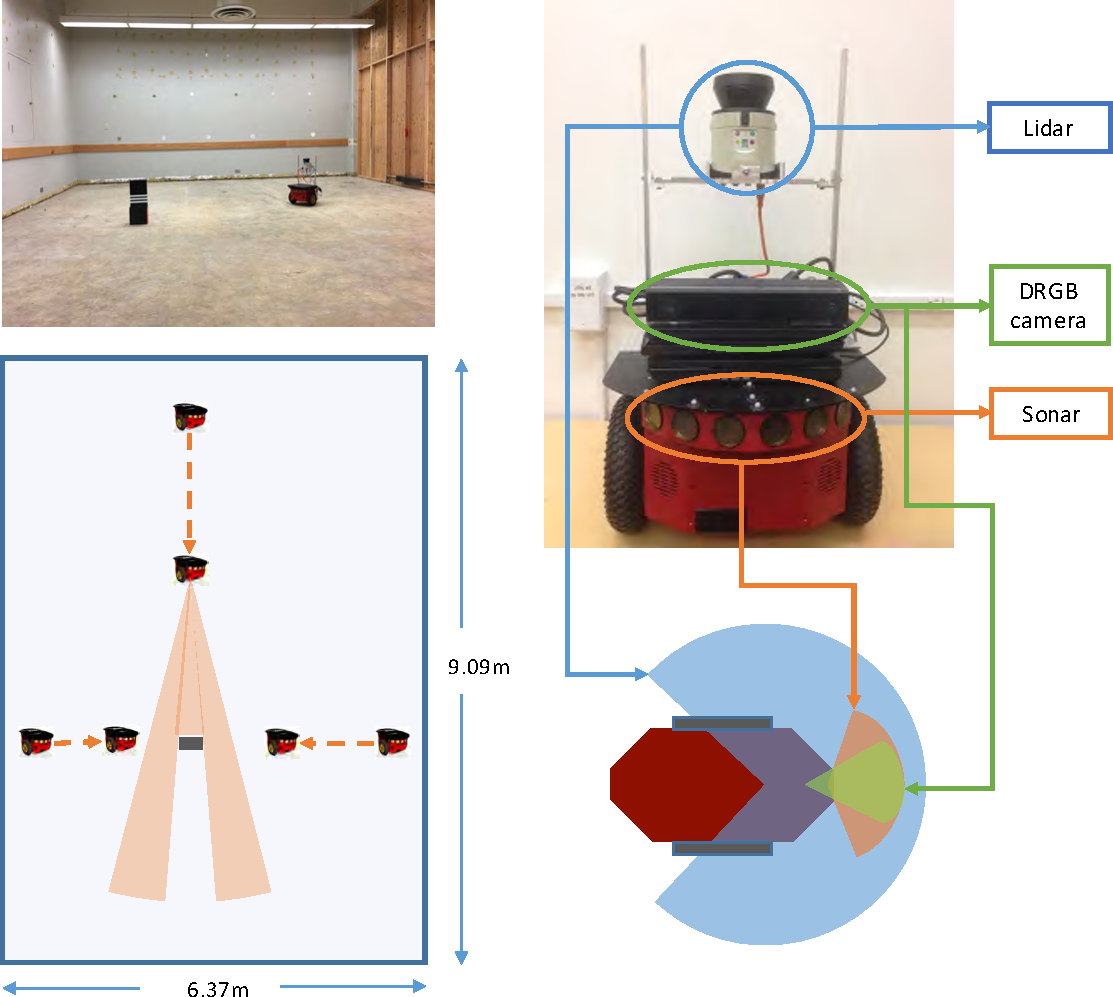
\includegraphics[width=0.4\textwidth]{exp_setup_rdsize_16-TIE-3798}%0.45
		\caption{Experiment Setup. Left: Three robots are used for localizing the target (black box). The room size is $9.09m\times 6.37m$. The orange sectors show the sonar sensing domain. Red dashed lines show the trajectory of each robot. Right: The mobile robot platform is equipped with different sensors. The sonar sensor is used for target localization.}\label{fig:exp_scene}
	\end{figure}
	
	\subsection{Moving UGVs, Moving Target}
	
	In this scenario, each UGV follows a pre-defined circular trajectory. 
	The target motion is modeled as a single-integrator with unit velocity on each direction.
	Each UGV executes the LIFO-DBF for moving target (\cref{subsec:LIFO-dbf-mov-tar}) for estimation.

	\cref{fig:htr_mov_sen_mov_tar_sing1,fig:htr_mov_sen_mov_tar_sing2,fig:htr_mov_sen_mov_tar_sing3,fig:htr_mov_sen_mov_tar_sing4} illustrate the evolution of individual PDF for the heterogeneous team.
	They present similar asymptotic behavior of individual PDFs as in previous simulations.	
	\cref{fig:htr_mov_sen_mov_tar_pos_err,fig:htr_mov_sen_mov_tar_entropy} compare LIFO-DBF with CbDF and CF.
	It is worth noting that CbDF achieves comparable position estimation error performance as the CF and LIFO-DBF.
	However, CbDF requires multiple rounds of exchanging individual PDFs, which incurs much higher communication burden than LIFO-DBF at each time step.
	Considering the small difference in position estimation error and significantly faster entropy reduction, LIFO-DBF is still preferable over CbDF for moving target scenario.
	
	\section{Indoor Experiment using Mobile Robot}\label{sec:exp}
	
	
	\begin{figure}
		\centering
		\begin{subfigure}[b]{0.21\textwidth}
			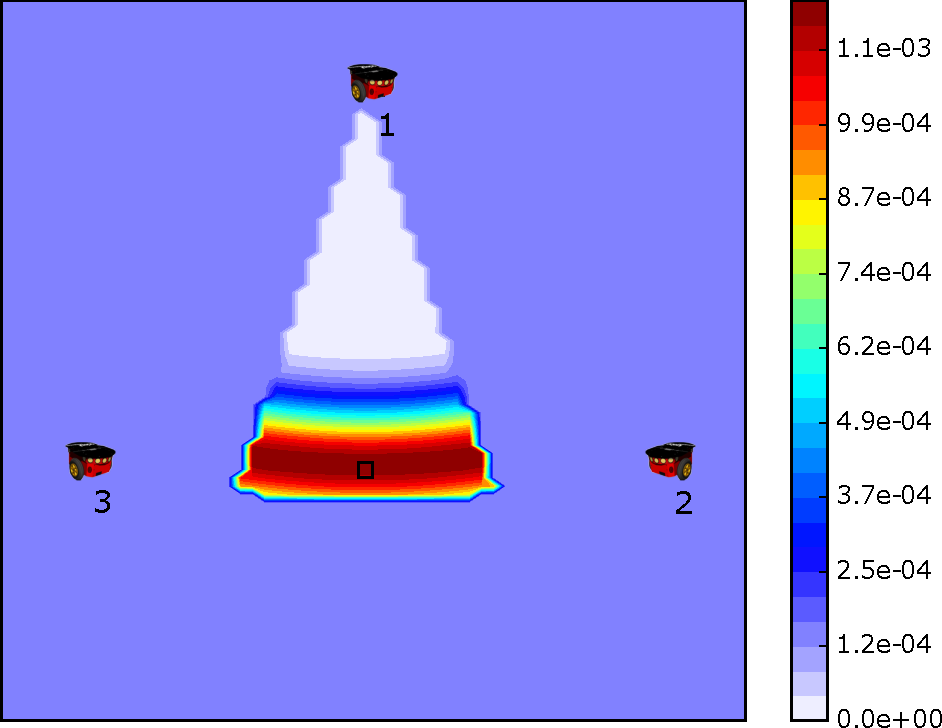
\includegraphics[width=\textwidth]{sonar_mov_sen_sta_tar_rbt1_step1_16-TIE-3798}
			\caption{Step 1}\label{fig:sonar_mov_sen_sta_tar_rbt1_step1}
		\end{subfigure}
		\begin{subfigure}[b]{0.21\textwidth}
			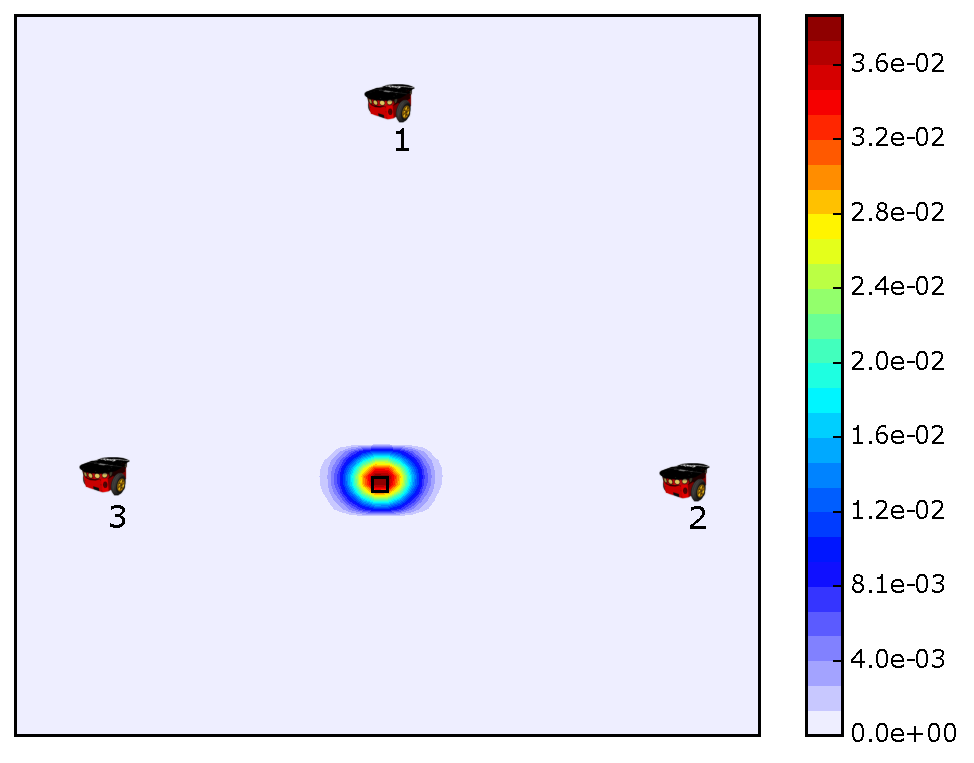
\includegraphics[width=\textwidth]{sonar_mov_sen_sta_tar_rbt1_step5_16-TIE-3798}
			\caption{Step 5}\label{fig:sonar_mov_sen_sta_tar_rbt1_step5}
		\end{subfigure}	
		\begin{subfigure}[b]{0.21\textwidth}
			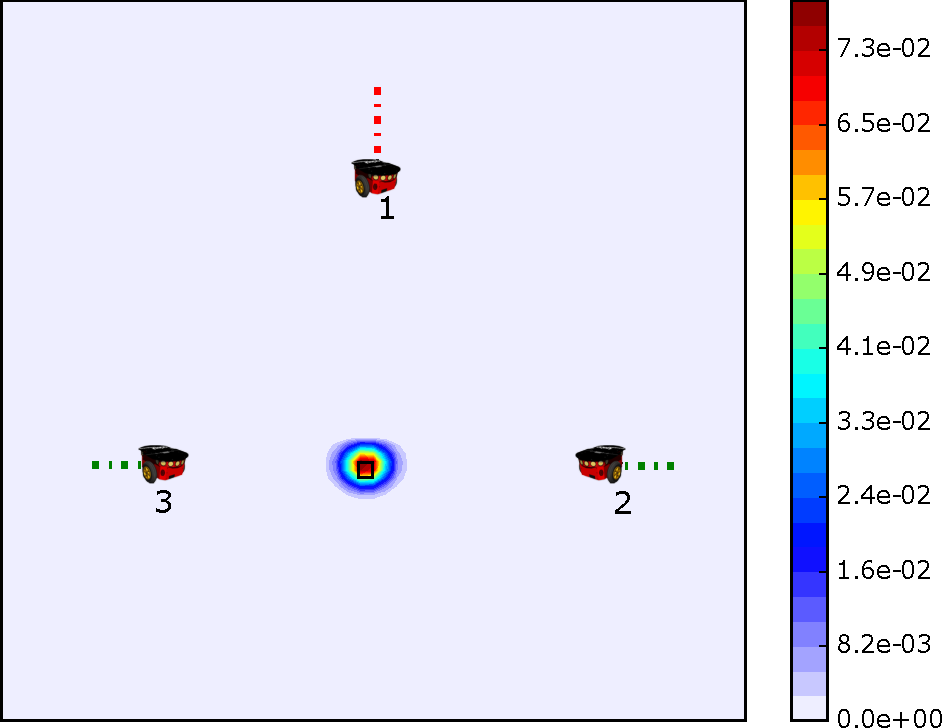
\includegraphics[width=\textwidth]{sonar_mov_sen_sta_tar_rbt1_step10_16-TIE-3798}
			\caption{Step 10}\label{fig:sonar_mov_sen_sta_tar_rbt1_step10}
		\end{subfigure}	
		\begin{subfigure}[b]{0.21\textwidth}
			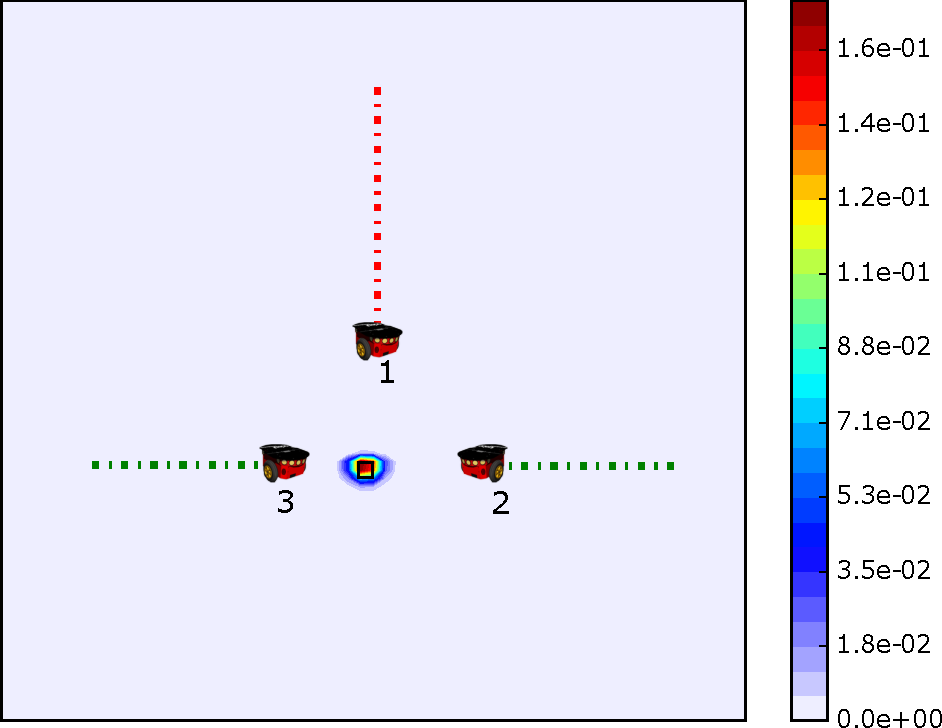
\includegraphics[width=\textwidth]{sonar_mov_sen_sta_tar_rbt1_step20_16-TIE-3798}
			\caption{Step 20}\label{fig:sonar_mov_sen_sta_tar_rbt1_step20}
		\end{subfigure}	
		\begin{subfigure}[b]{0.21\textwidth}
			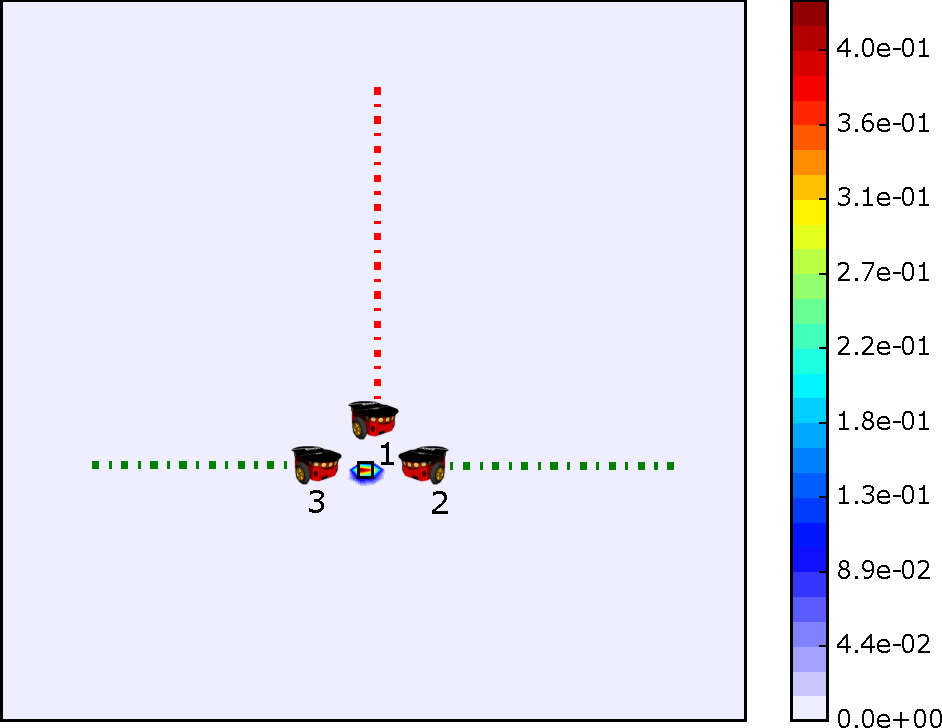
\includegraphics[width=\textwidth]{sonar_mov_sen_sta_tar_rbt1_step30_16-TIE-3798}
			\caption{Step 30}\label{fig:sonar_mov_sen_sta_tar_rbt1_step30}
		\end{subfigure}	
		\begin{subfigure}[b]{0.21\textwidth}
			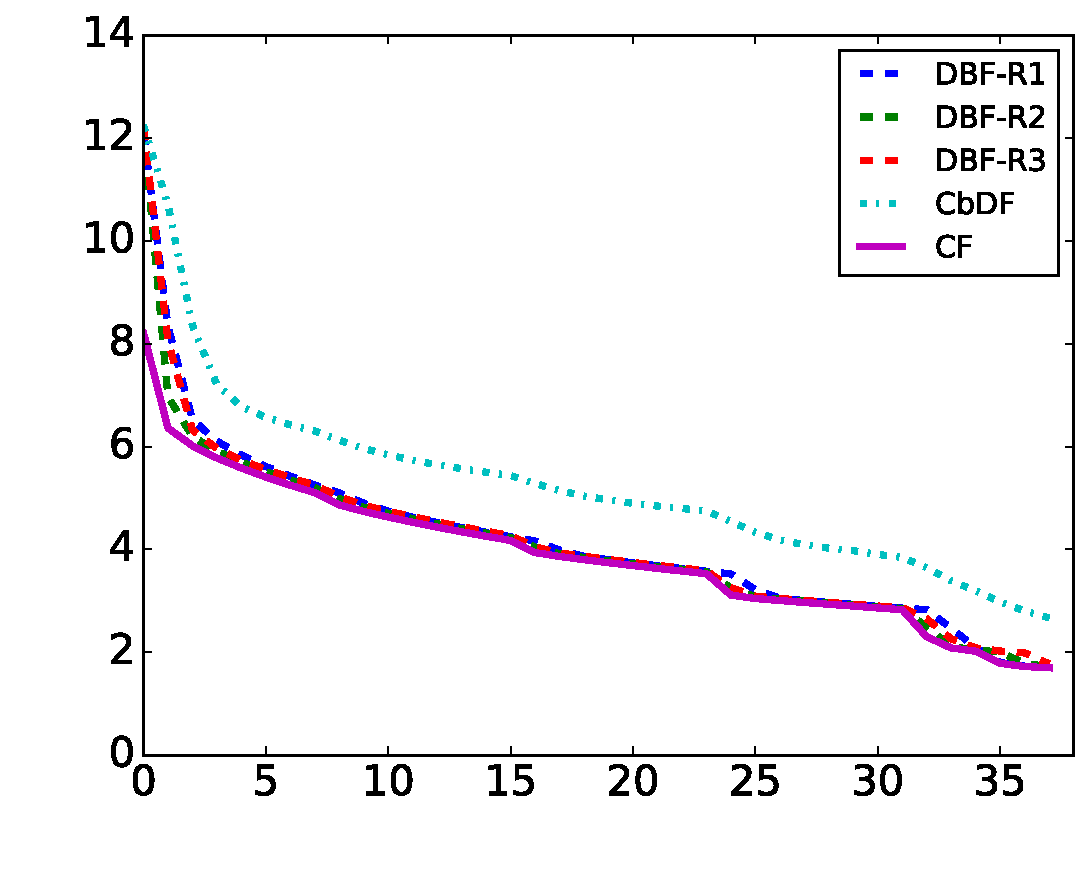
\includegraphics[width=\textwidth]{sonar_entropy_modified_16-TIE-3798}
			\caption{Entropy of Individual PDF}\label{fig:sonar_entropy}
		\end{subfigure}	
		\caption{The $1^\text{st}$ robot's individual PDF at different time steps.}
	\end{figure}
	
	
	We have conducted a target localization experiment to validate the LIFO-DBF approach in an indoor environment.
	The experiment equipments are illustrated in \cref{fig:exp_scene}.
	\textcolor{black}{Each robot is equipped with an onboard sonar sensor to measure the target (a small cardboard box) position.}
	The sonar sensor has the sensing field of view of $25\degree$ and the range of $4.9m$.
	Its measurement noise is modeled as a zero-mean Gaussian random variable with standard deviation $0.51m$.
	\textcolor{black}{The robots locally run the LIFO-DBF to estimate the target position. Each robot's probability map is constructed on an evenly spaced grid with $0.1m$ interval on each axis.
		In the experiment, robots move to different locations to measure the target position.
		We manually measure the robot positions where the sensor measurements are obtained to reduce the effects of localization error.}
	The effect of the target size has been compensated during the post-processing of the measurement data.
	
	\cref{fig:sonar_mov_sen_sta_tar_rbt1_step1,fig:sonar_mov_sen_sta_tar_rbt1_step5,fig:sonar_mov_sen_sta_tar_rbt1_step10,fig:sonar_mov_sen_sta_tar_rbt1_step20,fig:sonar_mov_sen_sta_tar_rbt1_step30} show the evolution of the $1^\text{st}$ robot's individual PDF.
	At step $1$, the probability mass concentrates to a stripe due to the fact that the sonar sensor used in this experiment has limited FOV and noise in range measurement.
	As new measurements from different robots are continually fused, the probability mass gradually concentrates to the true position of the target. 
	\textcolor{black}{Similar to previous simulations, we compare our method with CbDF and CF.
		All three approaches achieve accurate position estimation.
		However, they differ in the uncertainty reduction, as shown in \cref{fig:sonar_entropy}.
		The CF has the fastest entropy reduction and the LIFO-DBF achieves comparable performance, while the CbDF shows the slowest entropy reduction.}
	These experiment results validate the consistency of LIFO-DBF and demonstrate its effectiveness for distributed filtering.
	
	\section{CONCLUSION}\label{sec:conclu}
	This paper presents a measurement dissemination-based distributed Bayesian filtering (DBF) approach for a multi-UGV network, utilizing the Latest-In-and-Full-Out (LIFO) protocol for measurement exchange.
	By communicating the communication buffers among neighboring UGVs, LIFO significantly reduces the transmission burden between each pair of UGVs to scale linearly with the network size.
	Two types of LIFO-DBF algorithms are proposed to estimate individual PDFs for static target and moving target, respectively.
	The consistency of LIFO-DBF is proved by utilizing the law of large numbers, which ensures that the estimated target position converges in probability to the true target position.
	The LIFO-DBF is compared with the consensus filter and the centralized filter in various simulations.
	Results have shown that LIFO-DBF achieves very similar performance as the centralized filter and is advantageous over the consensus filter.
	An experiment is also conducted and has demonstrated the effectiveness of LIFO-DBF for distributed filtering.
	\textcolor{black}{The LIFO-DBF is promising for a wide range of applications using multiple robots, such as the environment monitoring, precision farming, and vehicle localization and mapping.}
	
	This work has opened up several directions for future work.
	\textcolor{black}{First, we plan to extend the current LIFO-DBF to deal with some common issues in the measurement for networked unmanned vehicles, including the asynchronous clock, communication delay, dynamically changing network, and packet loss.
		Second, LIFO-DBF provides a general framework for distributed nonlinear filtering. 
		In our future work, we will develop computationally efficient implementation of LIFO-DBF by using particle filters and Unscented Kalman filters.
		Lastly, we will combine the distributed filtering with path planning approaches \cite{liu2015model} so that multiple robots can actively localize and track targets, which can be applied to search and rescue and the navigation of autonomous vehicles.}
	
	\addtolength{\textheight}{0cm}   % This command serves to balance the column lengths
	% on the last page of the document manually. It shortens
	% the textheight of the last page by a suitable amount.
	% This command does not take effect until the next page
	% so it should come on the page before the last. Make
	% sure that you do not shorten the textheight too much.
	
	%%%%%%%%%%%%%%%%%%%%%%%%%%%%%%%%%%%%%%%%%%%%%%%%%%%%%%%%%%%%%%%%%%%%%%%%%%%%%%%%
	
	
	
	%%%%%%%%%%%%%%%%%%%%%%%%%%%%%%%%%%%%%%%%%%%%%%%%%%%%%%%%%%%%%%%%%%%%%%%%%%%%%%%%
	
	
	
	%%%%%%%%%%%%%%%%%%%%%%%%%%%%%%%%%%%%%%%%%%%%%%%%%%%%%%%%%%%%%%%%%%%%%%%%%%%%%%%%
	
	\section*{ACKNOWLEDGMENT}
	This article is in memory of Prof. J Karl Hedrick, who dedicated valuable time to contributing to this work while he was fighting with cancer. 
	His intellectual contribution to nonlinear control and transportation engineering and his dedication to students and colleagues has always inspired, and will continue inspiring us to explore the unknown and educate the next generation of scholars.
	
	%%%%%%%%%%%%%%%%%%%%%%%%%%%%%%%%%%%%%%%%%%%%%%%%%%%%%%%%%%%%%%%%%%%%%%%%%%%%%%%%
	% note: IEEEtranTIE seems have some issues. I need to use \bibliographystyle{IEEEtran} to generate bibliographies, and then use \bibliographystyle{IEEEtranTIE}.
	\bibliographystyle{IEEEtran}
	%\bibliographystyle{bibtex}
	\bibliography{references}
	
%	{\color{black}
%		
%			\vspace{-1cm}
%		\begin{IEEEbiography}[{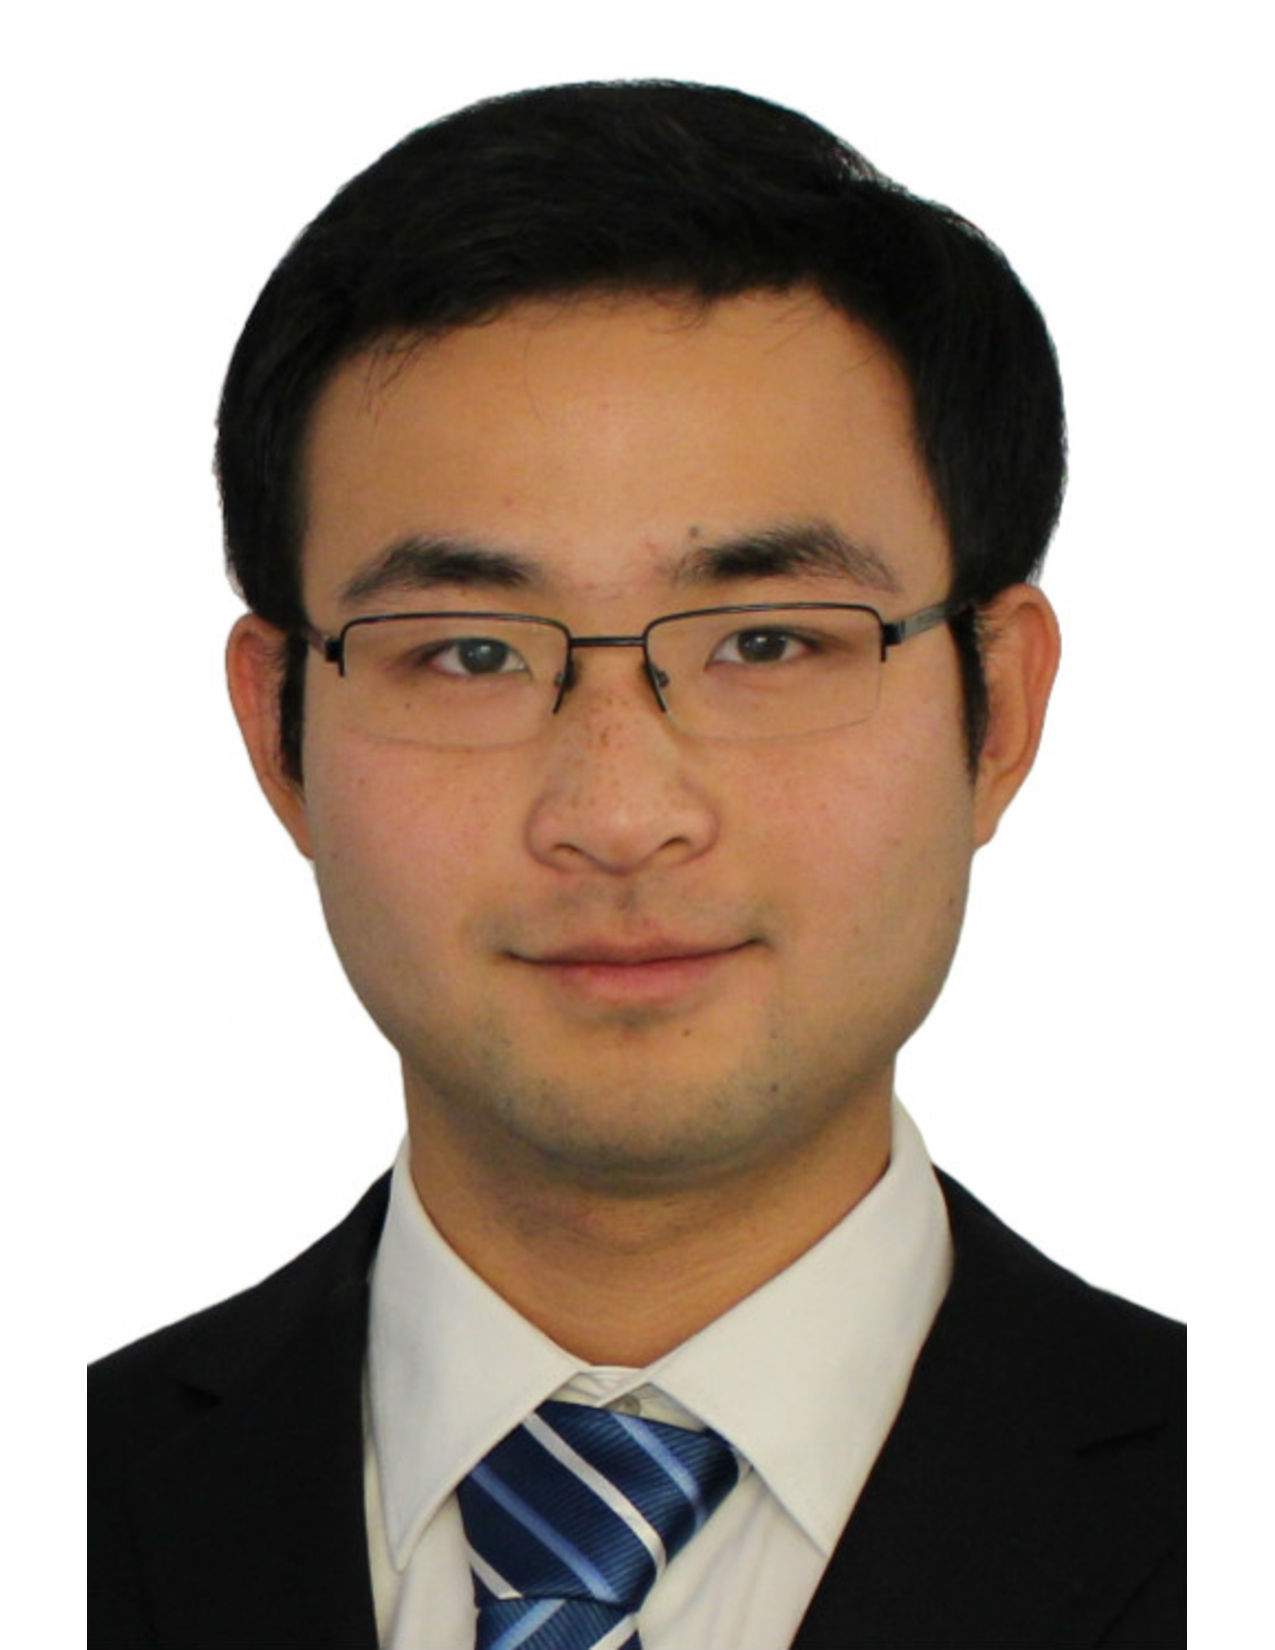
\includegraphics[width=1in,height=1.25in,clip,keepaspectratio]{Author_ChangLiu}}]
%			{Chang Liu} (S'15) received the B.S. degree in Electrical Engineering and in Applied Mathematics (double major) in 2011 from Peking University, China. He received the M.S. degree in Mechanical Engineering and in Computer Science in 2014 and 2016 from the University of California, Berkeley, USA. He is currently working towards the Ph.D. degree in Mechanical Engineering. 
%			
%			He is a Graduate Student Researcher with the Vehicle Dynamics and Control Laboratory, University of California, Berkeley, headed by Prof. J. Karl Hedrick and Prof. Francesco Borrelli. His research interests include robot path planning, distributed filtering, and human–--robot collaboration.
%
%		\end{IEEEbiography}
%		
%		\vspace{-1.3cm}
%		\begin{IEEEbiography}[{
\includegraphics[width=1in,height=1.25in,clip,keepaspectratio]{Author_ShengboLi}}]
%			{Shengbo Eben Li} received the M.S. and Ph.D. degrees from Tsinghua University in 2006 and 2009. He is currently the associate professor in Department of Automotive Engineering at Tsinghua University. 
%			
%			His active research interests include autonomous vehicle control, learning-based driver assistance, distributed control and optimal estimation, etc. He is the author of over 100 journal/conference papers, and the co-inventor of over 20 patents. Dr. Li was the recipient of Best Student Paper Award in 2014 IEEE Intelligent Transportation System Symp., Best Paper Award in 14th ITS Asia Pacific Forum (2015), Excellent Young Scholar of NSF China (2016), Yangtze River Scholar –Excellent Young Professor (2016). He served as the TPC member of IEEE Intelligent Vehicle Symposium, ISC member of FAST-zero 2017 in Japan, associated editor of IEEE ITSM and IEEE ITS, etc.\\ 
%		\end{IEEEbiography}
%		
%		\vspace{-1.3cm}
%		\begin{IEEEbiography}[{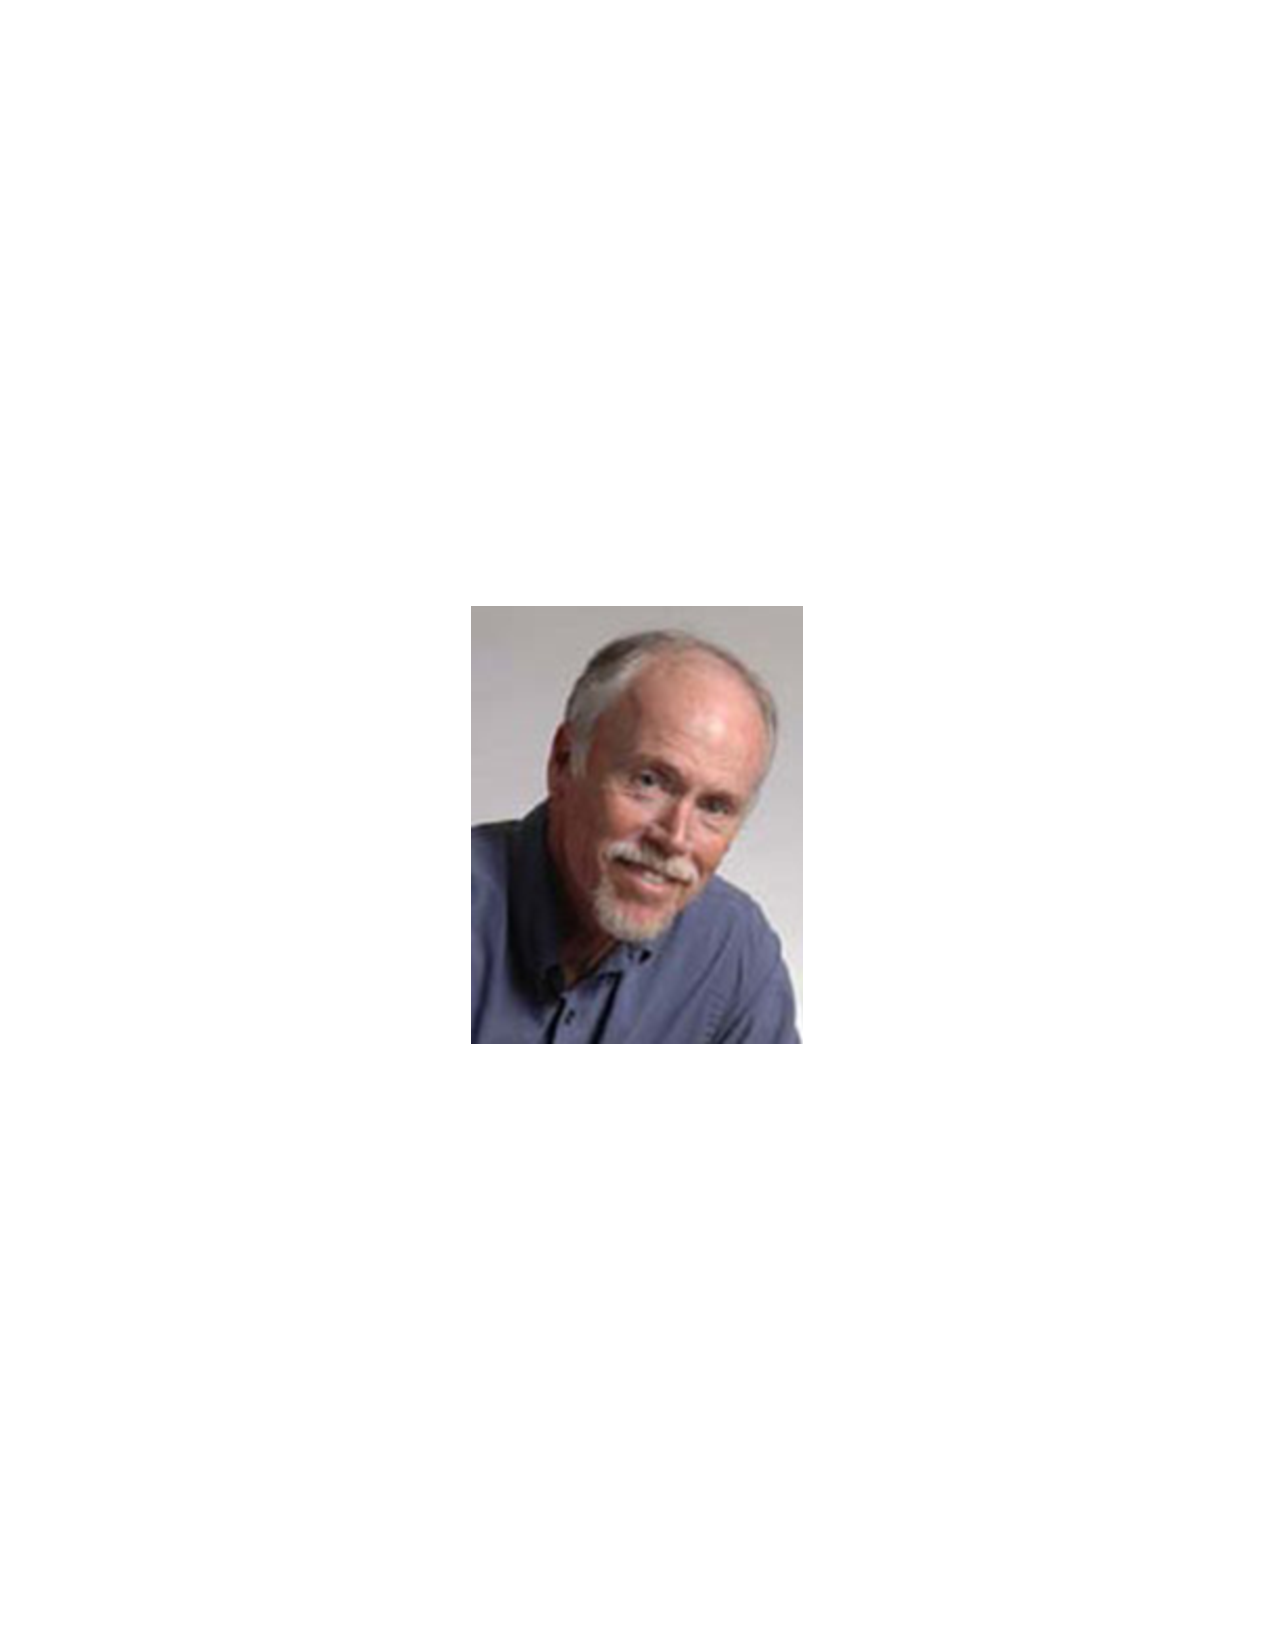
\includegraphics[width=1in,height=1.25in,clip,keepaspectratio]{Author_JKarlHedrick}}]
%			{J. Karl Hedrick} received the B.S. degree in Engineering Mechanics from University of Michigan, Ann Arbor, MI, USA, in 1966 and the M.S. and Ph.D. degrees in Aeronautical and Astronautical Engineering from Stanford University, Stanford, CA, USA, in 1970 and 1971, respectively.
%			
%			He is the James Marshall Wells Professor of mechanical engineering with the Department of Mechanical Engineering, University of California, Berkeley, CA, USA. His research interests include nonlinear control and its application to transportation systems.
%			\\ \\ 
%		\end{IEEEbiography}
%	}
	
\end{document}